\documentclass[11pt, a4paper, titlepage]{ltjsarticle}
\usepackage{geometry}
\usepackage{cite}
\usepackage{url}
%\usepackage[dvipdfmx]{graphicx} 
%[dvipdfmx]が悪さしてる
\usepackage{graphicx}
\usepackage[subrefformat=parens]{subcaption}
\usepackage{ulem}
\geometry{left=25mm,right=25mm,top=25mm,bottom=30mm}

\title{
2024年度 応用プログラミング実験\\
ディジタル信号処理\\
レポート}
\author{
学修番号: 22140025 \\
氏名: 稲村怜於奈 \\
}
\begin{document}
\date{
第1回レポート提出日(修正あり):2024/06/13 \\
第2回レポート提出日(修正あり):2024/06/20 \\
第3回レポート提出日:2024/06/27 \\
}
\maketitle

\section*{はじめに}

\subsection*{実験の概要}
(本実験の概要を書く.)
第1回の実験では1次元信号のフーリエ変換を行う.
MATLAB上でアナログ正弦波
$x_{T_{0}}(t)=A\sin(2\pi F_{0}t+\theta)+ D$
を定義し,$x_{T_{0}(t)}$から標本間隔$T_{s}$を
1/8[sec]として$n=0,1,\dots,7$まで8点標本化した有限な
離散時間信号$x[n]$を生成する.この方法で生成した
離散時間信号$x[n]$は8点と粗い間隔で標本化を行っている.
そこで次に,細かい標本間隔$(T_{sa}=1/1000)$を用い,
アナログ正弦波$x_{T_{0}}(t)$を疑似的に生成した$x(t)$を扱う.
その上で$x(t)$と$x[n]$とを$0\leq t < 1,0 \leq n < 8$
の範囲でグラフに重ねてプロットし,$x[n]$の点の位置と
$x(t)$の点の位置とが一致していることを確認する.
離散時間信号$x[n]$を$N=8$点DFTし,離散フーリエスペクトル
$X[k]$を求める.ただし第1回の実験ではDFTを行う祭際に
FFTを用いる.求めた$X[k]$の振幅スペクトル$|X[k]|$および
位相スペクトル$\angle X[k]$ [rad]をそれぞれ
$k=0,1,\dots ,N-1$の範囲でグラフにプロットする.
そのとき振幅スペクトルの横軸を周波数インデックス$k$に
対応する$F$[Hz]とし,位相スペクトルの横軸を周波数インデックス
$k$に対応する$\Omega$[rad/sec]とする.
FFTで使った周波数インデックス$k$に対応する$\omega$[rad],
$f$,$\Omega$[rad/sec],$F$[Hz]の値を表にしてまとめる.
この手順で課題1-1から1-5は$A,T_{0},\theta,D$の値を変えて行い,
課題1-6は 基本周期$T_{0}=1$[sec]の周期アナログ信号が
$a_{T_{0}}(t)=2\sin(2\pi t)+\sin(4\pi t+\pi)$
を同じように標本化する.課題1-7では課題1-1の手順を基本周期
$T_{0}=0.8$とした離散時間信号を$x[n]$として実行する.
追加課題では$N=20$とし,$0\leq t \leq N/2$の時$y(t)=1$,$t>N/2$の時
$y(t)=0$の短形波$y(t)$を$N$点FFTする.\\

第2回の実験ではMATLAB上で2種類の和音を重ねた二和音を作成し,
その二和音に対して様々な
ディジタルフィルタをかける.課題2-1では
正弦波$x(t)=\sin(2\pi F_{a}t)$
から標本化した離散時間信号を使って,MATLAB上で和音を表現する.
第1回の実験で行ったように正弦波$x(t)=\sin(2\pi F_{a}t)$から
サンプリングされた離散時間信号$x_{1}[n],(n=0,1,\dots,N-1)$
を生成する.そのとき(ラ)$F_{a}=440$[Hz]とする.また,以降は標本化
周波数は$F_{s}=2000$[Hz],すなわち時刻$t=n/2000$[sec]で標本化
されるとし,サンプリングの点数$N$は1秒間に該当する$N=F_{s}$
とする.次に$F_{a}$の値を先ほどと異なる周波数のものにして新たな
単音$x_{2}[n]$を生成する.今回は(ド)$F_{a}=261.626$とする.
$x_{1}[n]$と$x_{2}[n]$の和信号$x_{add}[n]$を生成し,MATLAB
上で再生して和音を確認する.生成した離散時間信号
$x_{1}[n],x_{2}[n],x_{add}[n]$の冒頭の20点分のみを1つの
グラフに重ねてプロットする.

課題2-2では2-1で生成した離散時間信号$x_{1}[n],x_{2}[n],x_{add}[n]$
の周波数成分を解析するために,各信号に$N=2000$のFFTをかけ,
得られた振幅スペクトル$|X[k]|$を信号毎に分けて図示する.
横軸は非正規化周波数$F=kF_{s}/N$[Hz]とする.

課題2-3では課題2-2で生成した離散時間信号$x_{add}[n]$に
ローパスフィルタをかけていく.周波数仕様の$F_{s}$を2000とし,
振幅仕様の単位を線形に,ローパスフィルタの遮断周波数
$F_{cut}=400$[Hz]となるようにする.通過域端周波数Fpassを
阻止域端周波数Fstopを非正規周波数で設定する.
生成したローパスフィルタ$h_{lpf}[n]$を$N=2000$点FFTし,
振幅スペクトル$|H_{lpf}[k]|$をグラフにする.ローパスフィルタ
$h_{lpf}[n]$に合成和音$x_{add}[n]$を畳み込み,畳み込み和
$y[n]$を得る.この畳み込み和$y[n]$の音を出力し,$N=2000$
点FFTし,振幅スペクトル$|Y[k]|$を確認する.
振幅スペクトルを示す場合横軸を非正規周波数$F=kF_{s}/N$[Hz]
で示す.

課題2-4では課題2-3と同じようにローパスフィルタだけでなく,
ハイパスフィルタやバンドパスフィルタなど様々なディジタルフィルタ
を生成する.任意の合成和音を生成し,任意のフィルタを用いて
畳み込み和の信号を生成する.

追加課題2-Aではdps2\_org.wavにノイズが加わったdps2\_noise.wav
のノイズ除去をする.FFTをして振幅スペクトルを求め,ノイズが
どのようなものか分析する.そしてそれに合うディジタルフィルタを
設計してノイズを除去する.

第3回の実験では標本化定理と窓関数について実験していく.
課題3-1では4Hzの正弦波を32点で標本化した離散時間信号
$x_{32}[n],(n=0,1,\dots,31)$を図示し,その離散フーリエスペクトル
$X_{32}[k]$を求めて,その振幅スペクトル$|X_{32}[k]|$を確認する.
次に標本化点数を6点とした離散時間信号$x_{6}[n](n=0,1,\dots,5)$
に対し,その離散フーリエスペクトル$X_{6}[k]$を求めて,その振幅スペクトル
$|X_{6}[k]|$を確認する.

課題3-2では逆フーリエ変換を行うことでDFTが変換対であること
を確認する.そのために,課題3-1で求めた離散時間フーリエスペクトル
$X_{32}[k]$および$X_{6}[k]$を用いてそれぞれの時間信号を求め
図示する.

課題3-3では窓関数の使い方とその効果を確かめる.まず,
4Hzの正弦波と6Hzの正弦波を合成し,32点で標本化した離散時間信号
$x_{add}[n],(n=0,1,\dots,31)$を生成し,32点DFTの結果
の振幅スペクトルを図示する.次に合成した離散時間信号
$x_{add}[n]$から$n=7,\dots,29$までの23点を切り出した信号を
離散時間信号$x_{cut}[n]$とし,23点DFTの結果の振幅スペクトル
を図示する.その次に切り出した離散時間信号$x_{cut}[n]$に
長さ23のハニング窓をかけた離散信号$x_{w}[n]$の23点DFTの結果
の振幅スペクトルを図示する.
ハニング窓とは
$x_{n}[n]=0.5-0.5\cos\left(\frac{2\pi n}{N-1}\right)$で
表される窓関数のことである.

追加課題3-Aでは
第 1 回の追加課題 1-A で用いた矩形波 $y(t)$ を $N = 200$ にして FFT を実行し,そのまま逆フーリエ変換で
戻した結果と,第 2 回のときと同じ手順でローパスフィルタ(設計は自由)を適用してから逆フーリエ変換を
行って戻した結果を比較する.



\subsection*{実験環境}
(使用したプログラミング言語など,本実験に用いた環境を書く.)\\
本実験はmatlab\footnote{https://jp.mathworks.com/products/matlab.html}を使って
デジタル信号処理の実験を行う.\\
11th Gen Intel (R) Core (TM) i5-1135G7
\footnote{https://www.intel.co.jp/content/www/jp/ja/products/sku/208658/intel-core-i51135g7-processor-8m-cache-up-to-4-20-ghz/specifications.html} 
@ 2.40 GHz   2.42 GHz
\\主記憶: Double Data Rate 4 Synchronous Dynamic Random-Access Memory
\footnote{https://www.jedec.org/standards-documents/docs/jesd79-4a},
 3200 MHz, 8 GB

\newpage
\section*{課題1-1}
%(課題 1-1 のレポートを記載する.多くの図をレポートに記載する必要があるので,下記のように横に並べて配置するなど工夫すること.ミス防止のためにも\textbackslash labelを使うことが望ましい.)
\subsection*{実験結果}
図\ref*{fign:sa1-1}に
$x_{T_{0}}(t)=A\sin(2\pi F_{0}t+\theta)+ D$に
$A=1,T_{0}=1,\theta=0,D=0$を代入したアナログ信号とそれを
標本化した標本値信号$x[n]$
の結果を,図\ref*{fign:sp1-1}に
$x[n]$をDFTした離散フーリエスペクトル$X[k]$
の結果を示す.表\ref*{t1}はFFT時で使った周波数インデックス
$k$に対応する$\omega$[rad],$f$,$\Omega$[rad/sec],$F$[Hz]の値
である.


\begin{figure}[h]
\begin{center}
\begin{minipage}[t]{0.48\columnwidth}
    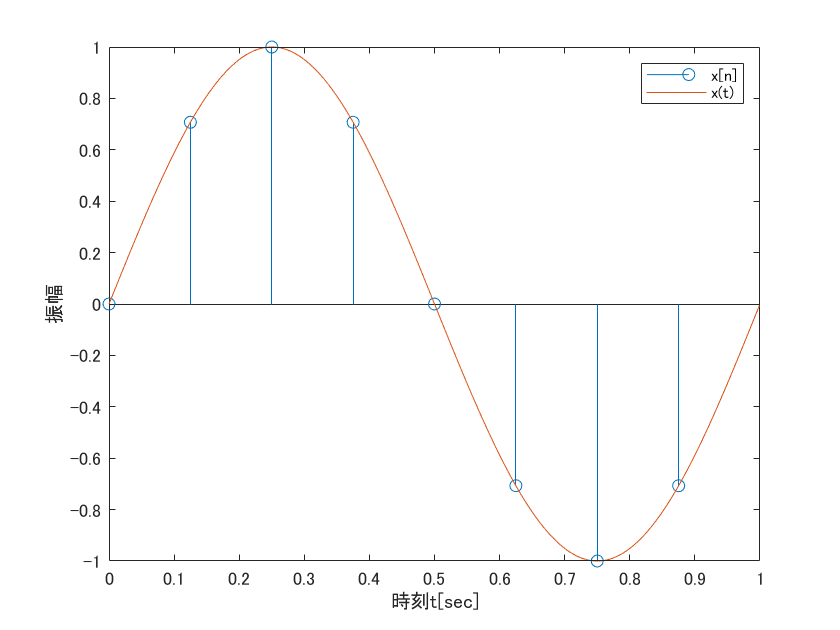
\includegraphics[width=\columnwidth]{figures/sampling1-1.png}
    \subcaption{周期アナログ信号$x_{T_{0}}(t)$(グラフ中ではx(t))
    とそれを標本化した標本値信号$x[n]$}
    \label{fign:sa1-1}
\end{minipage}
\begin{minipage}[t]{0.48\columnwidth}
    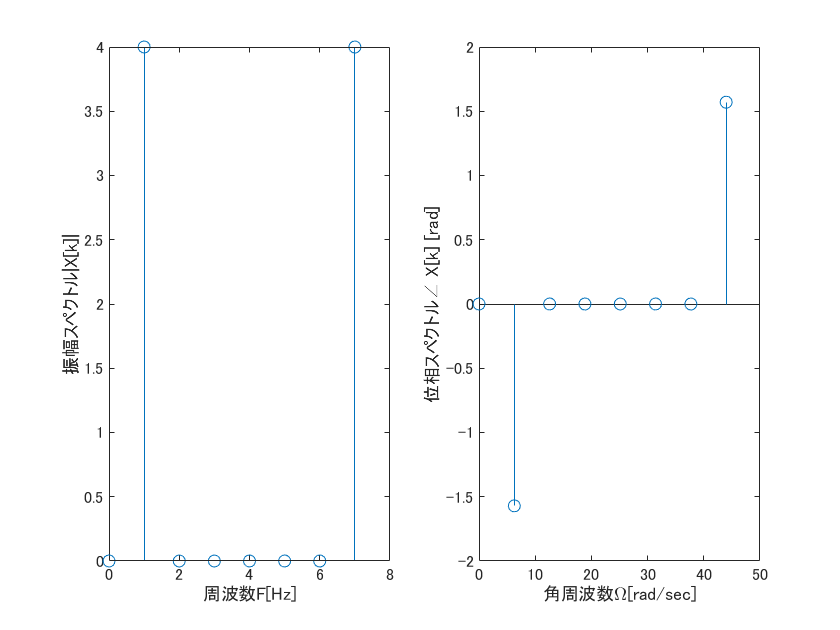
\includegraphics[width=\columnwidth]{figures/spectrum1-1.png}
    \subcaption{離散フーリエスペクトル$X[k]$}
    \label{fign:sp1-1}
\end{minipage}
\end{center}
\caption{\sout{課題1-1で得られたグラフ}
$x_{T_{0}}(t)=\sin(2\pi t)$を8点で標本化した信号とそれをDFTした離散フーリエスペクトル}
\end{figure}
\begin{table}[h]
    \centering
    \caption{周波数インデックスと各変数の対応表}
    \begin{tabular}{crrrrrrrr}
  \hline
  $k$&0&1&2&3&4&5&6&7\\
  $\omega$ [rad]&0&	0.7854	&1.5708	&2.3562	&3.1416	&3.9270	&4.7124	&5.4978\\
  $f$&0&0.1250&0.2500&	0.3750&	0.5000&	0.6250&	0.7500&	0.8750\\
  $\Omega$ [rad/sec]&0&	6.2832&12.5664&18.8496&25.1327&31.4159&37.6991&43.9823\\
  $F$ [Hz]&0&	1&	2&	3&	4&	5	&6&	7\\
  \hline

    \end{tabular}
    \label{t1}
\end{table}
\subsection*{考察}
図\ref*{fign:sa1-1}より,標本化した$x[n]$の点の位置と
アナログ信号の$x(t)$の点の位置が一致している.
これは$x[n]$が$x(t)$を標本化して作られたためである.したがって
標本化するとアナログ信号上から標本点の分だけ取り出すということ
ができるとわかる.また,図\ref*{fign:sp1-1}を見ると
$F=1,F=7$のところで振れ幅スペクトルが非0になっている.
$N$点離散フーリエ変数は次式で表される.\\
$\displaystyle X[k] = \sum_{n=0}^{N-1}x[n]\exp
\left(-\frac{j2\pi nk}{N}\right),k=0,1,\dots,N-1$\\
この式の複素数$X[k]$は離散フーリエス
ペクトルと呼ばれ,信号$x[n]$に含まれる正規化角周波数$2\pi k/N$ [rad]の複素指数信号の振幅$|X[k]|$
や位相$\angle X[k]$などの情報を与える.なお,$X[k]$は$\omega=2\pi k/N$ [rad]の離散時間フーリエスペクト
ル$X(e^{j\omega})$と等しい.また,$\exp(-j2\pi nk/N)=\exp{j2\pi n(k-N)/N}$より,$X[k]=X[(k-N)]$
である.$F=1,F=7$のところで振れ幅スペクトルが同じになったのは
今回$N=8$で$X[k]=X[(k-8)]$なので$X[7]=X[7-8]=X[-1]$
となり,振幅スペクトルは偶対称であるためである.同様に
位相スペクトルが$X[1],X[7]$で逆位相になっているのは
位相スペクトルが奇対称であるためである.
$F=1$のところにあるのは$T_{0}=1$で$F_{0}=1$となり,周波数
が1になっているからである.

\newpage
\section*{課題1-2}
\subsection*{実験結果}
図\ref*{fign:sa1-2}に
$x_{T_{0}}(t)=A\sin(2\pi F_{0}t+\theta)+ D$に
$A=1,T_{0}=1/2,\theta=0,D=0$を代入したアナログ信号とそれを
標本化した標本値信号$x[n]$
の結果を,図\ref*{fign:sp1-2}に
$x[n]$をDFTした離散フーリエスペクトル$X[k]$
の結果を示す.
\begin{figure}[h]
\begin{center}
\begin{minipage}[t]{0.48\columnwidth}
    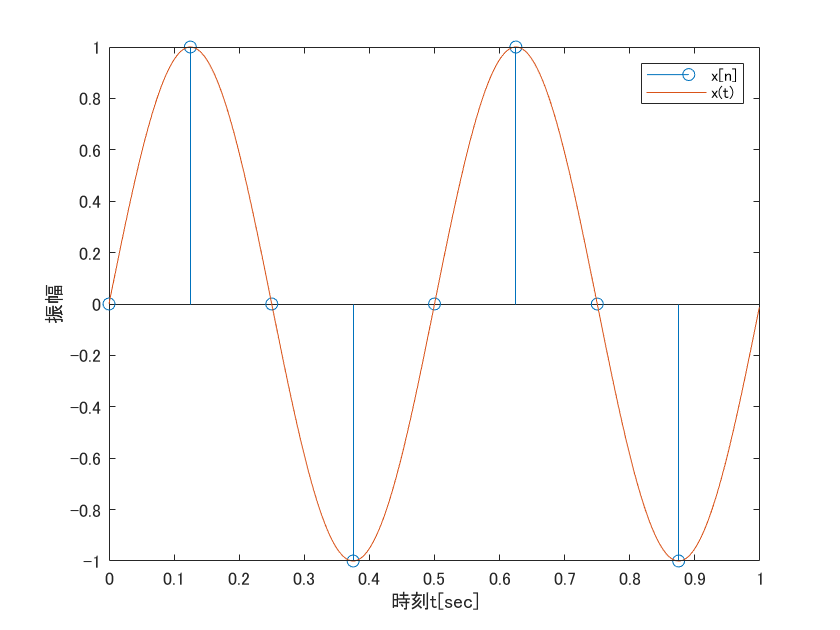
\includegraphics[width=\columnwidth]{figures/sampling1-2.png}
    \subcaption{周期アナログ信号$x_{T_{0}}(t)$(グラフ中ではx(t))
    とそれを標本化した標本値信号$x[n]$}
    \label{fign:sa1-2}
\end{minipage}
\begin{minipage}[t]{0.48\columnwidth}
    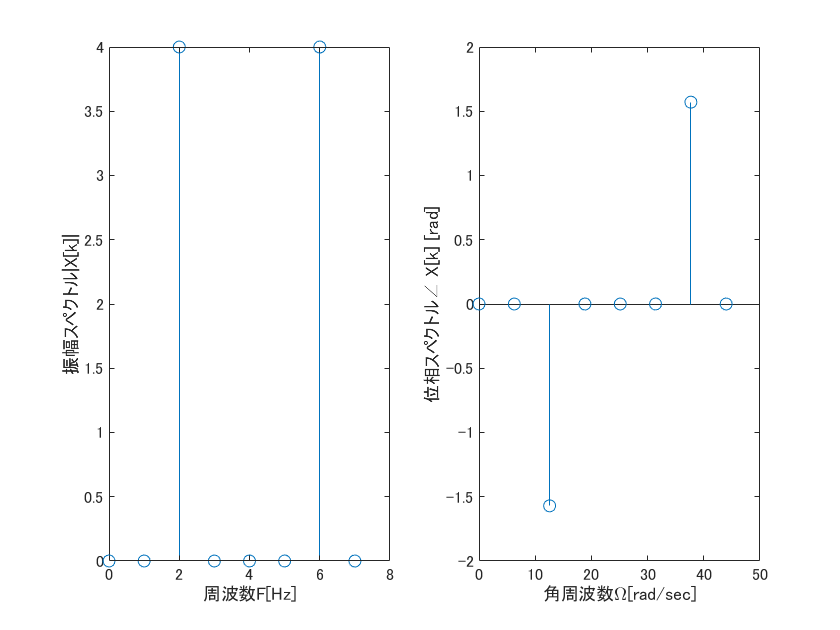
\includegraphics[width=\columnwidth]{figures/spectrum1-2.png}
    \subcaption{離散フーリエスペクトル$X[k]$}
    \label{fign:sp1-2}
\end{minipage}
\end{center}
\caption{\sout{課題1-2で得られたグラフ}
$x_{T_{0}}(t)=\sin(2\pi 2t)$を8点で標本化した信号とそれをDFTした離散フーリエスペクトル}
\end{figure}
\subsection*{考察}
図\ref*{fign:sa1-1}と図\ref*{fign:sa1-2}を比較すると,
実験1-2は周期が1/2倍になっている.
図\ref*{fign:sp1-1}と図\ref*{fign:sp1-2}を比較すると,
図\ref*{fign:sp1-1}は$F=1$の位置に,図\ref*{fign:sp1-2}は
$F=2$の位置に,それぞれスペクトルが存在している.これは
それぞれの信号の周波数が,1Hzと2Hzと異なっているためである.
したがって振幅スペクトルのスペクトルが存在する周波数が,
信号に含まれている周波数を示していることがわかる.



\newpage
\section*{課題1-3}
\subsection*{実験結果}
図\ref*{fign:sa1-3}に
$x_{T_{0}}(t)=A\sin(2\pi F_{0}t+\theta)+ D$に
$A=2,T_{0}=1,\theta=0,D=0$を代入したアナログ信号とそれを
標本化した標本値信号$x[n]$
の結果を,図\ref*{fign:sp1-3}に
$x[n]$をDFTした離散フーリエスペクトル$X[k]$
の結果を示す.
\begin{figure}[h]
\begin{center}
\begin{minipage}[t]{0.48\columnwidth}
    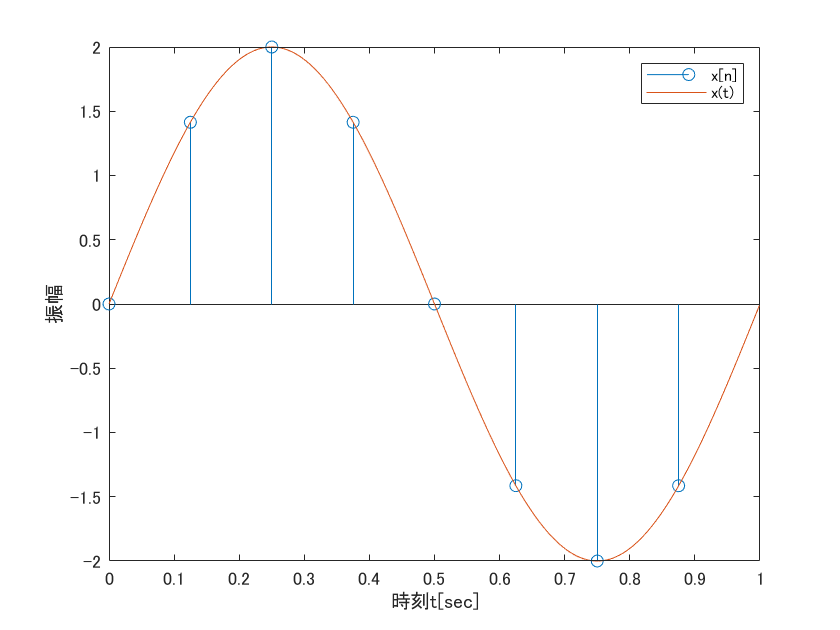
\includegraphics[width=\columnwidth]{figures/sampling1-3.png}
    \subcaption{周期アナログ信号$x_{T_{0}}(t)$(グラフ中ではx(t))
    とそれを標本化した標本値信号$x[n]$}
    \label{fign:sa1-3}
\end{minipage}
\begin{minipage}[t]{0.48\columnwidth}
    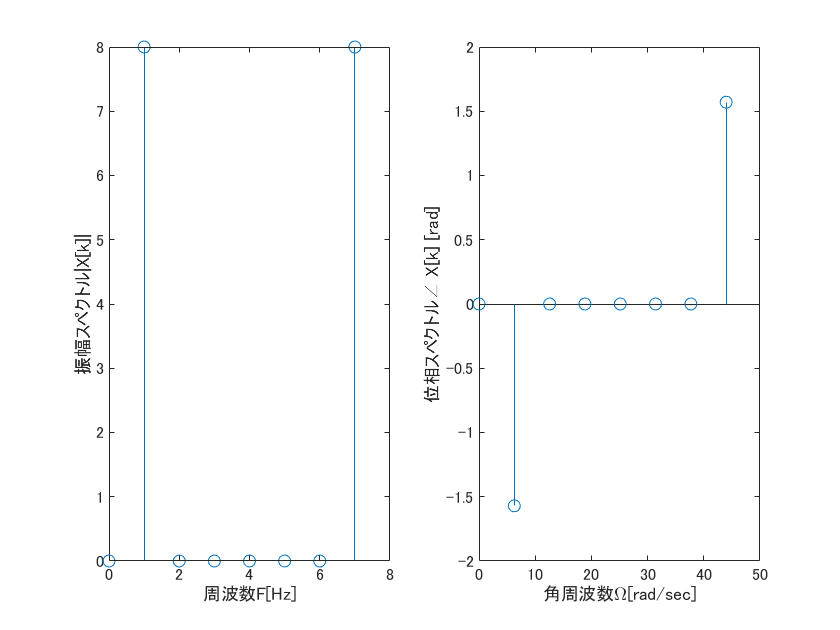
\includegraphics[width=\columnwidth]{figures/spectrum1-3.png}
    \subcaption{離散フーリエスペクトル$X[k]$}
    \label{fign:sp1-3}
\end{minipage}
\end{center}
\caption{\sout{課題1-3で得られたグラフ}
$x_{T_{0}}(t)=2\sin(2\pi t)$を8点で標本化した信号とそれをDFTした離散フーリエスペクトル}
\end{figure}
\subsection*{考察}
図\ref*{fign:sa1-1}と図\ref*{fign:sa1-3}を比較すると
振幅が2倍になっている.
図\ref*{fign:sp1-1}と図\ref*{fign:sp1-3}を比較すると,
図\ref*{fign:sp1-1}は振幅スペクトル$|X[k]|$の値が4に,図\ref*{fign:sp1-3}は
振幅スペクトル$|X[k]|$の値が8になっている.これは
それぞれの信号の振幅が,1と2と異なっているためである.
したがって振幅スペクトルのスペクトルの値が,
信号に含まれている振幅を示していることがわかる.
図\ref*{fign:sp1-2}と図\ref*{fign:sp1-3}を比較すると,
振幅スペクトルの値や位置が異なっているためである.
したがって振幅スペクトルのスペクトルの値や存在する周波数が
信号に含まれている振幅や周波数を示していることがわかる
\newpage
\section*{課題1-4}
\subsection*{実験結果}
図\ref*{fign:sa1-4}に
$x_{T_{0}}(t)=A\sin(2\pi F_{0}t+\theta)+ D$に
$A=1,T_{0}=1/2,\theta=\pi,D=0$を代入したアナログ信号とそれを
標本化した標本値信号$x[n]$
の結果を,図\ref*{fign:sp1-4}に
$x[n]$をDFTした離散フーリエスペクトル$X[k]$
の結果を示す.
\begin{figure}[h]
\begin{center}
\begin{minipage}[t]{0.48\columnwidth}
    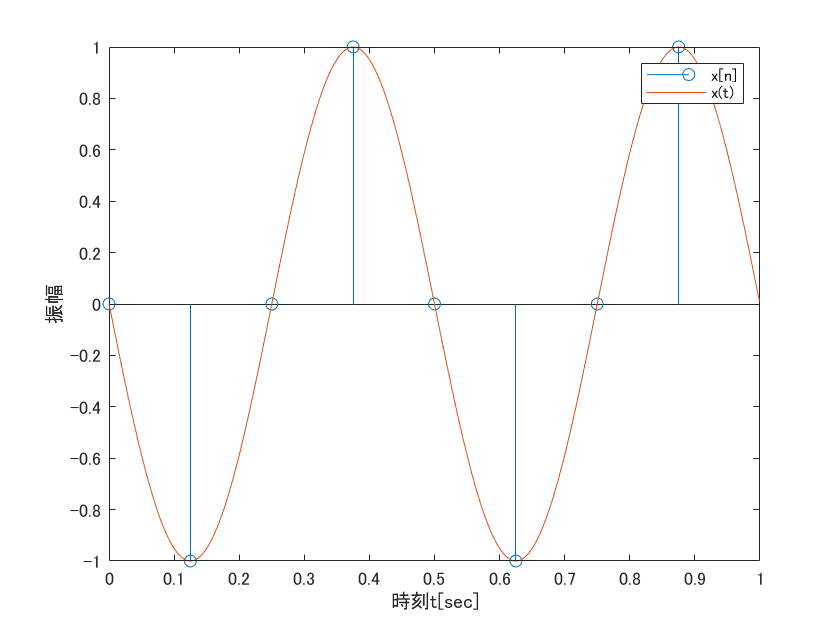
\includegraphics[width=\columnwidth]{figures/sampling1-4.png}
    \subcaption{周期アナログ信号$x_{T_{0}}(t)$(グラフ中ではx(t))
    とそれを標本化した標本値信号$x[n]$}
    \label{fign:sa1-4}
\end{minipage}
\begin{minipage}[t]{0.48\columnwidth}
    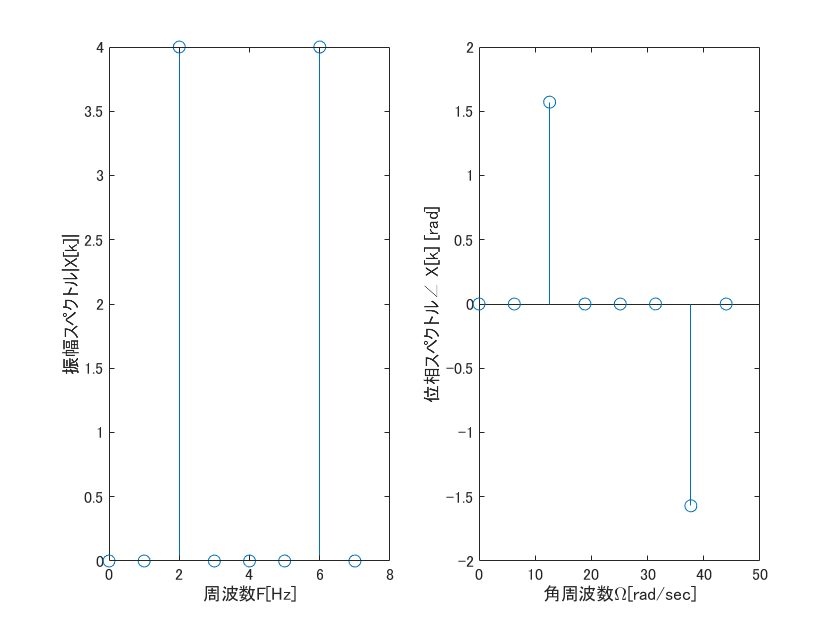
\includegraphics[width=\columnwidth]{figures/spectrum1-4.png}
    \subcaption{離散フーリエスペクトル$X[k]$}
    \label{fign:sp1-4}
\end{minipage}
\end{center}
\caption{\sout{課題1-4で得られたグラフ}
$x_{T_{0}}(t)=\sin(2\pi 2t+\pi)$を8点で標本化した信号とそれをDFTした離散フーリエスペクトル}
\end{figure}
\subsection*{考察}
図\ref*{fign:sa1-2}と図\ref*{fign:sa1-4}を比較すると
逆位相になっている.
図\ref*{fign:sp1-2}と図\ref*{fign:sp1-4}を比較すると,
図\ref*{fign:sp1-2}は位相スペクトル$\angle X[k]$の値が1.5に,図\ref*{fign:sp1-2}は
位相スペクトル$\angle X[k]$の値が-1.5になっている.これは
それぞれの信号の初期位相が,0と$\pi$と異なっているためである.
したがって位相スペクトルの値が,
信号に含まれている初期位相を示していることがわかる.
%%%%%%%%%%%%%%%%%%%%%%%%%%%%%
図\ref*{fign:sp1-1}と図\ref*{fign:sp1-4}を比較すると,
図\ref*{fign:sp1-1}は位相スペクトルの値や位置
が異なっている.これは
それぞれの信号の初期位相や周波数が異なっているためである.
したがって位相スペクトルの値,位置が,
信号に含まれている初期位相,周波数を示していることがわかる.
図\ref*{fign:sp1-3}と図\ref*{fign:sp1-4}を比較すると,
図\ref*{fign:sp1-3}は位相スペクトルの値,振幅スペクトルの値や位置
が異なっている.これは
それぞれの信号の初期位相や振幅,周波数が異なっているためである.
したがって位相スペクトルの値,振幅スペクトルの値や位置が,
信号に含まれている初期位相,振幅,周波数を示していることがわかる.
\newpage
\section*{課題1-5}
\subsection*{実験結果}
図\ref*{fign:sa1-5}に
$x_{T_{0}}(t)=A\sin(2\pi F_{0}t+\theta)+ D$に
$A=1,T_{0}=1,\theta=0,D=1$を代入したアナログ信号とそれを
標本化した標本値信号$x[n]$
の結果を,図\ref*{fign:sp1-5}に
$x[n]$をDFTした離散フーリエスペクトル$X[k]$
の結果を示す.
\begin{figure}[h]
\begin{center}
\begin{minipage}[t]{0.48\columnwidth}
    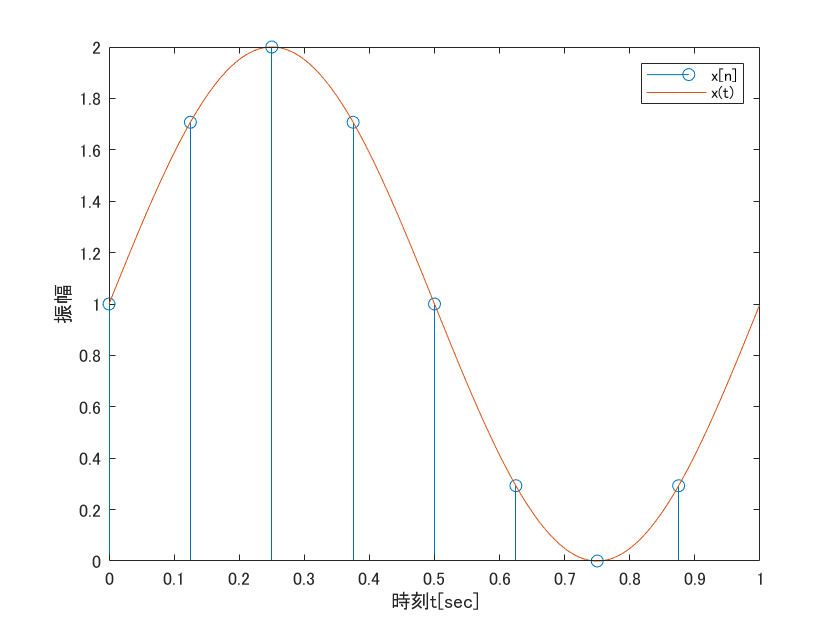
\includegraphics[width=\columnwidth]{figures/sampling1-5.png}
    \subcaption{周期アナログ信号$x_{T_{0}}(t)$(グラフ中ではx(t))
    とそれを標本化した標本値信号$x[n]$}
    \label{fign:sa1-5}
\end{minipage}
\begin{minipage}[t]{0.48\columnwidth}
    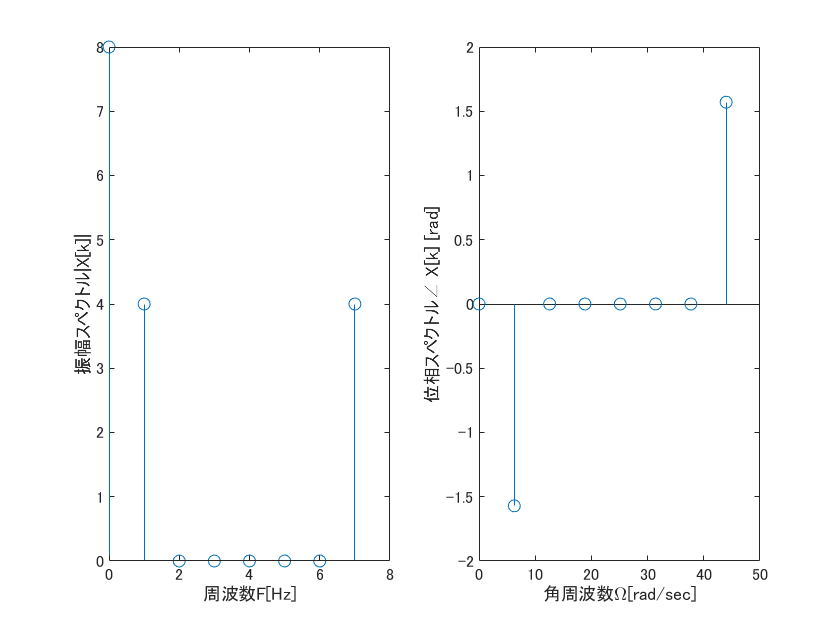
\includegraphics[width=\columnwidth]{figures/spectrum1-5.png}
    \subcaption{離散フーリエスペクトル$X[k]$}
    \label{fign:sp1-5}
\end{minipage}
\end{center}
\caption{\sout{課題1-5で得られたグラフ}
$x_{T_{0}}(t)=\sin(2\pi t)+1$を8点で標本化した信号とそれをDFTした離散フーリエスペクトル}
\end{figure}
\subsection*{考察}
図\ref*{fign:sa1-1}と図\ref*{fign:sa1-5}を比較すると,
実験1-2の値は実験1-1の値の全ての箇所で1足されている.
図\ref*{fign:sp1-1}と図\ref*{fign:sp1-5}を比較すると,
図\ref*{fign:sp1-1}は振幅スペクトル$|X[k]|$が8に,図\ref*{fign:sp1-5}は
振幅スペクトル$|X[k]|$が0に$F=0$のときなっている.これは
それぞれの信号の直流成分が,0と1と異なっているためである.
したがって$F=0$のときの振幅スペクトルの値が,
信号に含まれている直流成分を示していることがわかる.


\newpage
\section*{課題1-6}
\subsection*{実験結果}
図\ref*{fign:sa1-6}に基本周期$T_{0}$の
アナログ信号$a_{T_{0}}(t)=2\sin(2\pi t)+\sin(4\pi t+\pi)$
とそれを標本化した標本値信号$a[n]$
の結果を,図\ref*{fign:sp1-6}に
$a[n]$をDFTした離散フーリエスペクトル$X[k]$
の結果を示す.
\begin{figure}[h]
\begin{center}
\begin{minipage}[t]{0.48\columnwidth}
    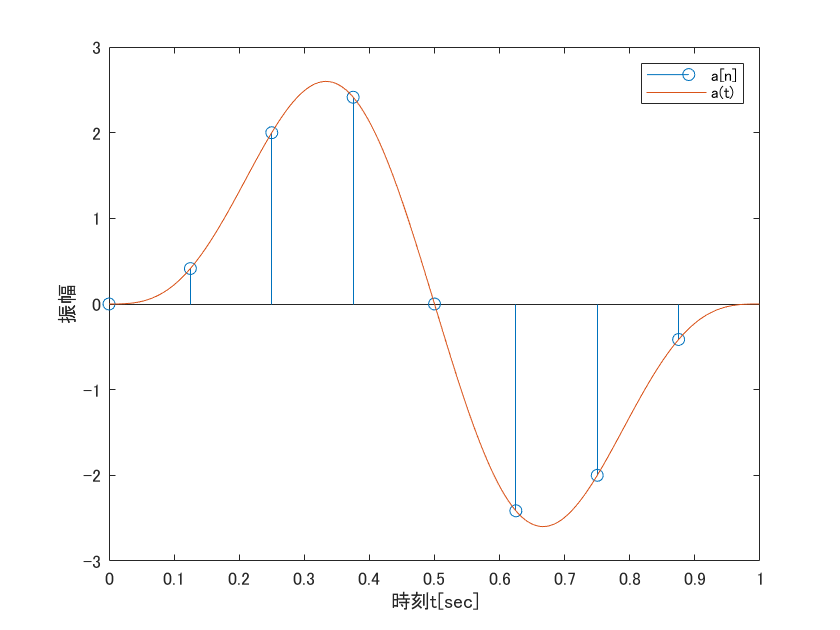
\includegraphics[width=\columnwidth]{figures/sampling1-6.png}
    \subcaption{周期アナログ信号$a_{T_{0}}(t)$(グラフ中ではa(t))
    とそれを標本化した標本値信号$a[n]$}
    \label{fign:sa1-6}
\end{minipage}
\begin{minipage}[t]{0.48\columnwidth}
    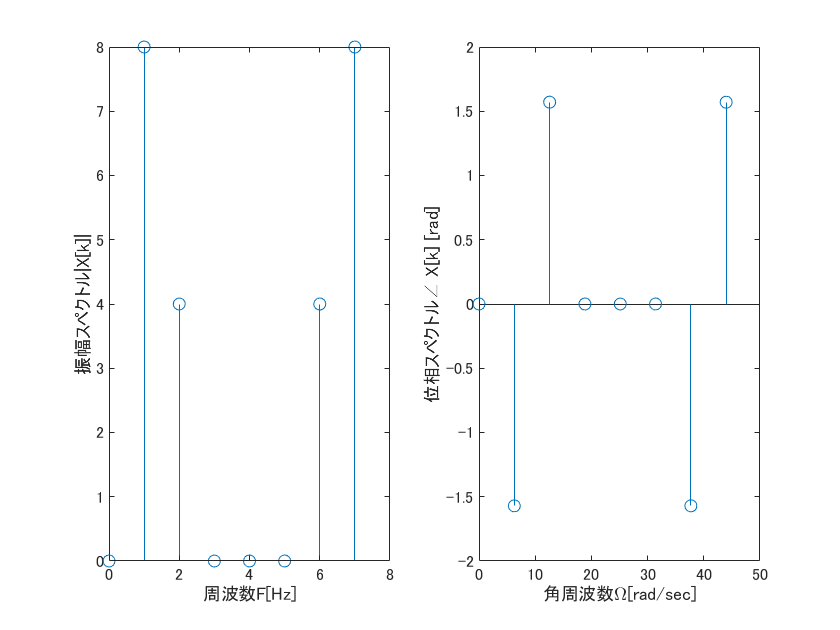
\includegraphics[width=\columnwidth]{figures/spectrum1-6.png}
    \subcaption{離散フーリエスペクトル$X[k]$}
    \label{fign:sp1-6}
\end{minipage}
\end{center}
\caption{\sout{課題1-6で得られたグラフ}
$x_{T_{0}}(t)=2\sin(2\pi t)+\sin(4\pi t + \pi)$を8点で標本化した信号とそれをDFTした離散フーリエスペクトル}
\end{figure}
\subsection*{考察}
図\ref*{fign:sa1-3}と図\ref*{fign:sa1-4}と図\ref*{fign:sa1-6}
を比較するとよく分からないが,
図\ref*{fign:sp1-3}と図\ref*{fign:sp1-4}と図\ref*{fign:sp1-6}
を比較すると実験1-6の離散フーリエスペクトルは
実験1-3と実験1-4を足し合わせて出来ている.
これは実験1-6のアナログ信号が$a_{T_{0}}(t)=2\sin(2\pi t)+\sin(4\pi t+\pi)$
であり,これは実験1-3,1-4の$2\sin(2\pi t)$,$\sin(4\pi t+\pi)$
を足すと出来上がるためである.
したがって離散フーリエスペクトルは複数の正弦波が足されている
信号でも正弦波ごとに分離してその信号がどんなものか理解しやすいことがわかる.
図\ref*{fign:sp1-2}と図\ref*{fign:sp1-4}と図\ref*{fign:sp1-6}
を比較すると実験1-6の離散フーリエスペクトルには
実験1-3が含まれて実験1-2の逆位相を足し合わせて出来ている.
これは前述のに加えて実験1-2は実験1-4の位相より$\pi$ずれている
ためである.



\newpage
\section*{課題1-7}
\subsection*{実験結果}
図\ref*{fign:sa1-1}に
$x_{T_{0}}(t)=A\sin(2\pi F_{0}t+\theta)+ D$に
$A=1,T_{0}=0.8,\theta=0,D=0$を代入したアナログ信号とそれを
標本化した標本値信号$x[n]$
の結果を,図\ref*{fign:sp1-1}に
$x[n]$をDFTした離散フーリエスペクトル$X[k]$
の結果を示す.
\begin{figure}[h]
\begin{center}
\begin{minipage}[t]{0.48\columnwidth}
    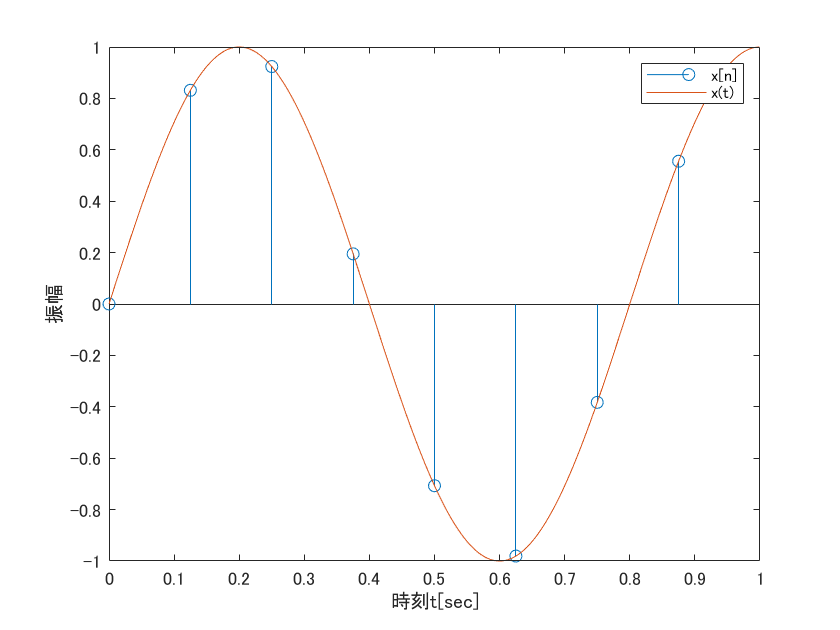
\includegraphics[width=\columnwidth]{figures/sampling1-7.png}
    \subcaption{周期アナログ信号$x_{T_{0}}(t)$(グラフ中ではx(t))
    とそれを標本化した標本値信号$x[n]$}
    \label{fign:sa1-7}
\end{minipage}
\begin{minipage}[t]{0.48\columnwidth}
    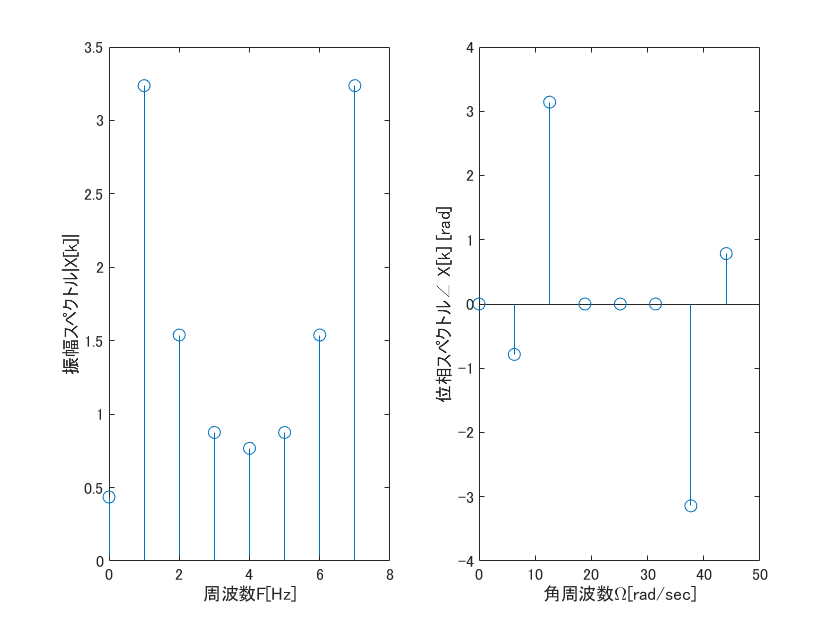
\includegraphics[width=\columnwidth]{figures/spectrum1-7.png}
    \subcaption{離散フーリエスペクトル$X[k]$}
    \label{fign:sp1-7}
\end{minipage}
\end{center}
\caption{\sout{課題1-7で得られたグラフ}
$x_{T_{0}}(t)=\sin(2\pi 1.25t)$を8点で標本化した信号とそれをDFTした離散フーリエスペクトル}
\end{figure}
\subsection*{考察}
図\ref*{fign:sp1-1}と図\ref*{fign:sp1-7}を比較すると,
図\ref*{fign:sp1-1}は,同じ$k$に対して二つ存在するが,
図\ref*{fign:sp1-7}は
振幅スペクトルがたくさんあって
その数に位相スペクトルの数があってない.
これは図\ref*{fign:sa1-1}と図\ref*{fign:sa1-7}を比較して
わかるように
実験1-7では基本周期$T_{0}$が0.8で$x[n]$が長さ$N=8$を周期とした
周期離散時間信号でないためである.
したがってDFTは周期離散時間信号の時にしか使えないことがわかる.
\newpage
\section*{課題1-A}
\subsection*{実験結果}
図\sout{\ref*{fign:sa1-A}}\ref*{fign:sa1-As}に$N=20$とし,
$0\leq t \leq N/2$の時$y(t)=1$,$t>N/2$の時
$y(t)=0$の短形波$y(t)$とそれを
標本化した標本値信号$y[n]$
の結果を,図\ref*{fign:sp1-A}に
$y[n]$を$N$点FFT\sout{する.}した離散フーリエスペクトル$X[k]$
の結果を示す.


\begin{figure}[h]
\begin{center}
\begin{minipage}[t]{0.48\columnwidth}
    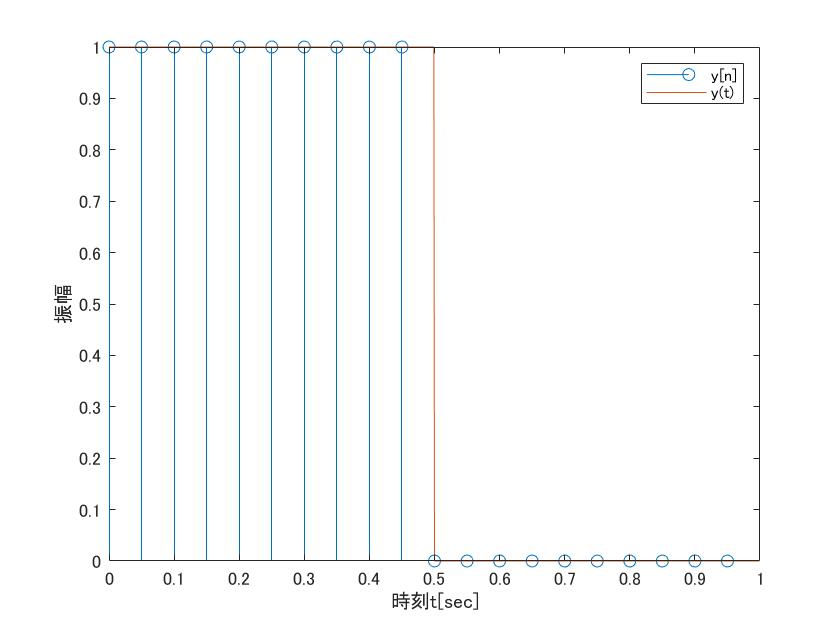
\includegraphics[width=\columnwidth]{figures/sampling1-A.png}
    \subcaption{\sout{周期アナログ信号$y_{T_{0}}(t)$(グラフ中ではy(t))
    とそれを標本化した標本値信号$y[n]$}}
    \label{fign:sa1-A}
\end{minipage}
\begin{minipage}[t]{0.48\columnwidth}
    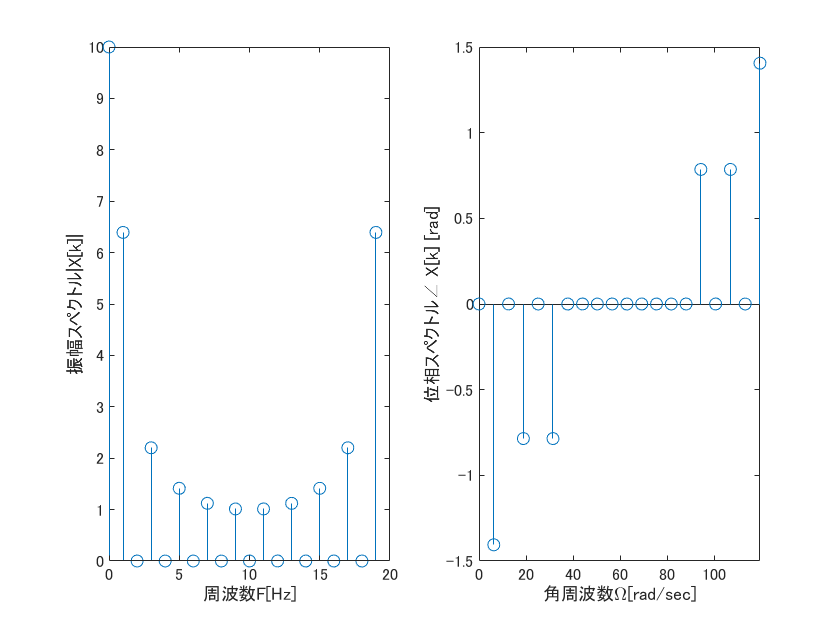
\includegraphics[width=\columnwidth]{figures/spectrum1-A.png}
    \subcaption{離散フーリエスペクトル$X[k]$}
    \label{fign:sp1-A}
\end{minipage}
\end{center}
\caption{\sout{課題1-Aで得られたグラフ}}
\end{figure}
\begin{figure}[h]
    \begin{center}
    \begin{minipage}[t]{0.48\columnwidth}
        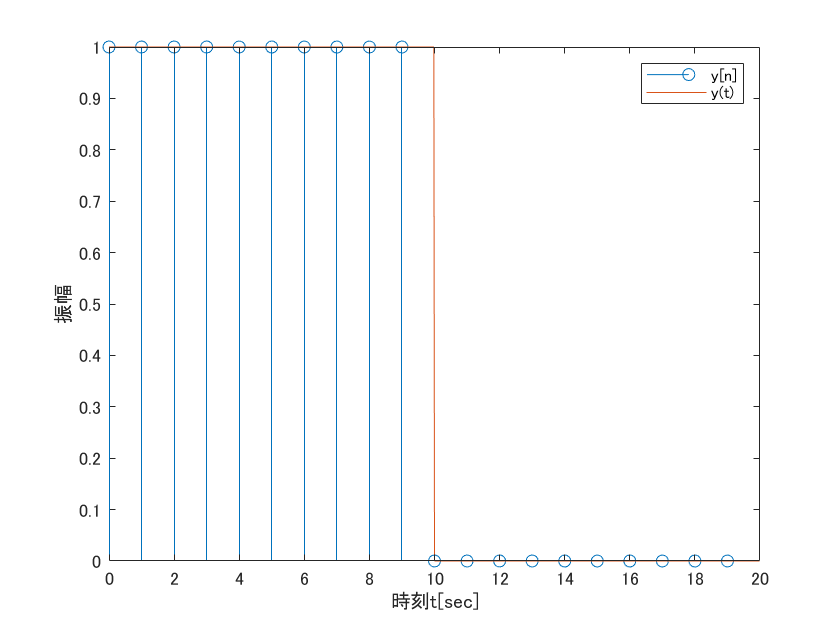
\includegraphics[width=\columnwidth]{figures/sampling1-A-syusei.png}
        \subcaption{周期アナログ信号$y_{T_{0}}(t)$(グラフ中ではy(t))
        とそれを標本化した標本値信号$y[n]$}
        \label{fign:sa1-As}
    \end{minipage}
    \begin{minipage}[t]{0.48\columnwidth}
        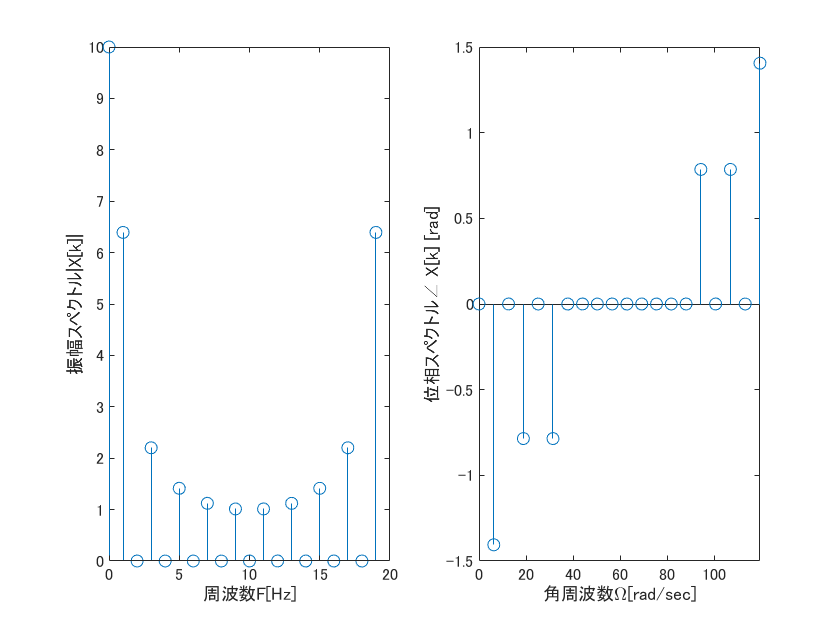
\includegraphics[width=\columnwidth]{figures/spectrum1-A.png}
        \subcaption{離散フーリエスペクトル$X[k]$}
        \label{fign:sp1-A}
    \end{minipage}
    \end{center}
    \caption{$N=20$とし,
$0\leq t \leq N/2$の時$y(t)=1$,$t>N/2$の時
$y(t)=0$の短形波$y(t)$を20点で標本化した信号とそれをDFTした離散フーリエスペクトル}
    \end{figure}
\subsection*{考察(追記あり)}
図\ref*{fign:sa1-1}と図\sout{\ref*{fign:sa1-A}}\ref*{fign:sa1-As}を比較すると,
形が違う.
図\ref*{fign:sp1-1}と図\ref*{fign:sp1-A}を比較すると,
図\ref*{fign:sp1-1}は,同じ$k$に対して二つ存在するが,
図\ref*{fign:sp1-A}は
振幅スペクトルがたくさんあって
その数に位相スペクトルの数があってない.
実験1-Aの$y(t)$の範囲では正弦波のように周期的になっていないためである.
したがってDFTは周期離散時間信号の時にしか使えないことがわかる.
また,振幅スペクトルが多く存在している.(
    特に低い周波数成分が多く高周波数成分は少なくなっている.
)これは$y(t)$のような波形
を作るには正弦波をたくさん足さなくては作れないためである.

\newpage
\section*{課題2-1}
\subsection*{実験結果}
今回は$x_{1}[n]$をラの$F_{a}=440.00$[Hz]
$x_{2}[n]$をドの$F_{a}=261.626$[Hz]として生成し,和信号
$x_{add}[n]$ を生成した.離散時間信号
$x_{1}[n],x_{2}[n],x_{add}[n]$の冒頭の20点分を図\sout{\ref*{fign:2-1}}
\ref*{fign:2-1s}
にプロットして示す.本来の信号は離散信号だが,見やすさの
観点から連続値として扱った.

\begin{figure}[h]
    \begin{center}
    \begin{minipage}[t]{0.48\columnwidth}
        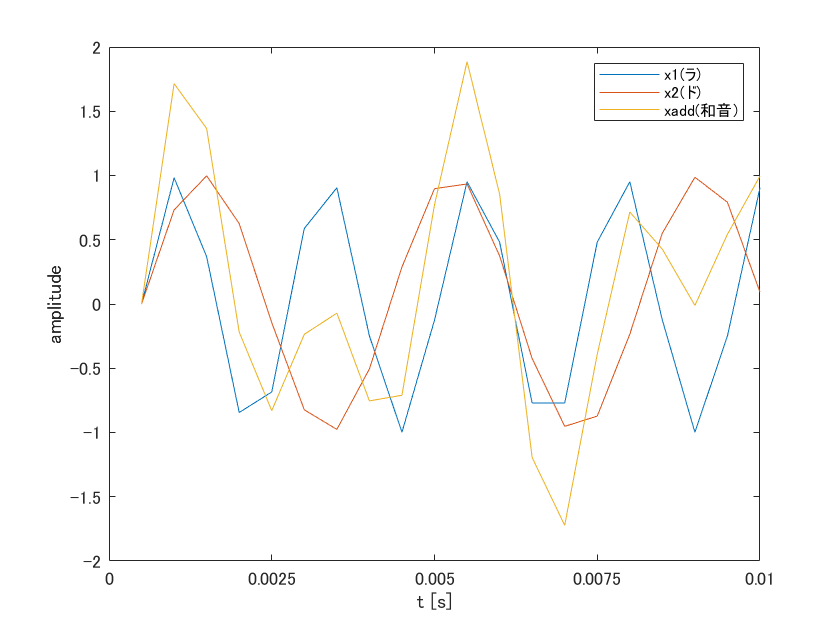
\includegraphics[width=\columnwidth]{figures/2-1.png}
        \subcaption{\sout{課題2-1で得られたグラフ}}
        \label{fign:2-1}  
    \end{minipage}
    \begin{minipage}[t]{0.48\columnwidth}
        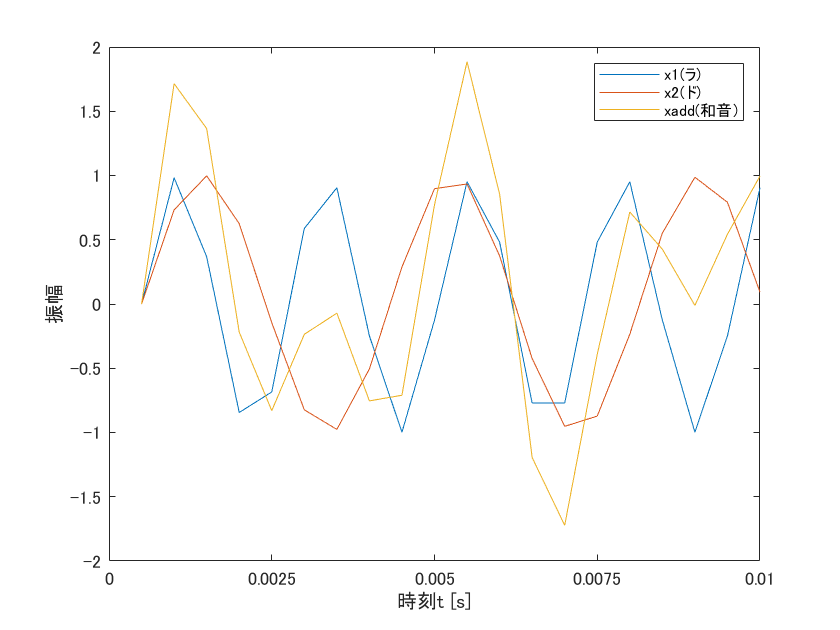
\includegraphics[width=\columnwidth]{figures/2-1-syusei.png}
        \subcaption{(ラ)の440Hzと(ド)の261.626Hzを合成した和音$x_{add}$の離散時間信号}
        \label{fign:2-1s}
    \end{minipage}
    \end{center}
    \caption{図の修正}
    \end{figure}
\newpage
\section*{課題2-2}
\subsection*{実験結果}
課題2-1で生成した離散時間信号$x_{1}[n],x_{2}[n],x_{add}[n]$
の周波数成分を解析するために,各信号に$N=2000$点のFFTをかけて
得られた振幅スペクトル$|X[k]|$を図\ref*{fign:2-2}に示す.
そのとき横軸を非正規周波数$F=kF_{s}/N$[Hz]とする.

\begin{figure}[h]
    \centering
    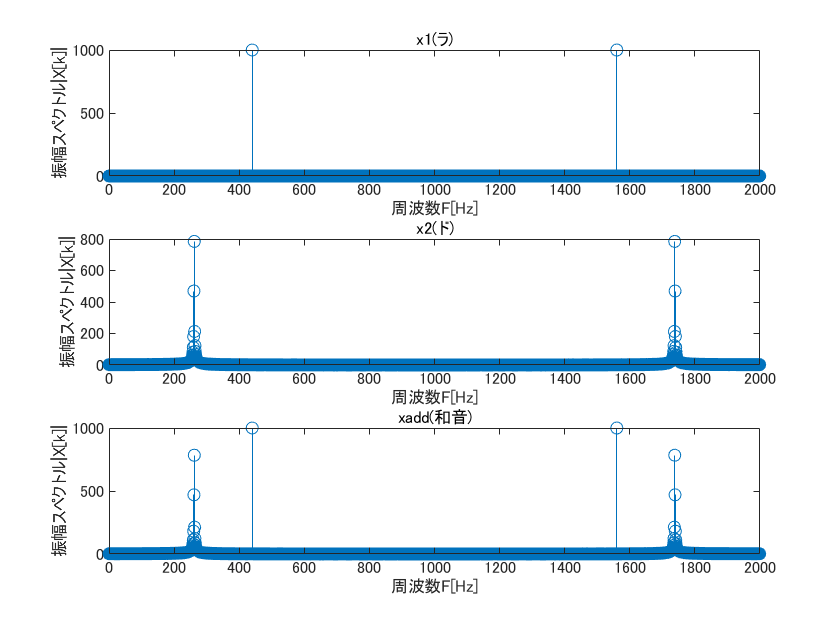
\includegraphics[width=0.9\linewidth]{figures/2-2.png}
    \caption{\sout{課題2-2で得られたグラフ}
    (ラ)の440Hzと(ド)の261.626Hzとそれらを合成した和音$x_{add}$の振幅スペクトル}
    \label{fign:2-2}     
\end{figure}
\subsection*{考察}
図\ref*{fign:2-2}より振幅スペクトルをみると,
$x_{1}[n]$と$x_{2}[n]$で振幅スペクトルが存在していた周波数
のところに,和音の$x_{add}[n]$でも同じ大きさで振幅スペクトル
が存在している.これは,$x_{add}[n]$は$x_{1}[n]$と$x_{2}[n]$
の和音だからである.したがって和音の周波数特性は
単音の周波数特性の和になっていると考えられる.

\newpage
\section*{課題2-3}
\subsection*{実験結果(追記あり)}
周波数仕様$Fs=2000$,遮断周波数$F_{cut}=400$[Hz]となるよう
通過域端周波数Fpassを380Hz,阻止域端周波数Fstopを420Hz
に設定してローパスフィルタ$h_{lpf}[n]$ を設計した.
設計したローパスフィルタ$h_{lpf}[n]$を$N=2000$点FFTし,
振幅スペクトル$|H_{lpf}[k]|$を図\ref*{fign:2-3lpf}
に示す.見やすさのために連続値として扱ってローパスフィルタを
プロットしている.
ローパスフィルタに(追記:課題2-1で生成した)合成和音$x_{add}[n]$を畳み込む.
そうして出来た畳み込み和$y[n]$を$N=2000$点FFTし,
振幅スペクトル$|Y[k]|$を図\ref*{fign:2-3y}
に示す.


\begin{figure}[h]
    \begin{center}
    \begin{minipage}[t]{0.48\columnwidth}
        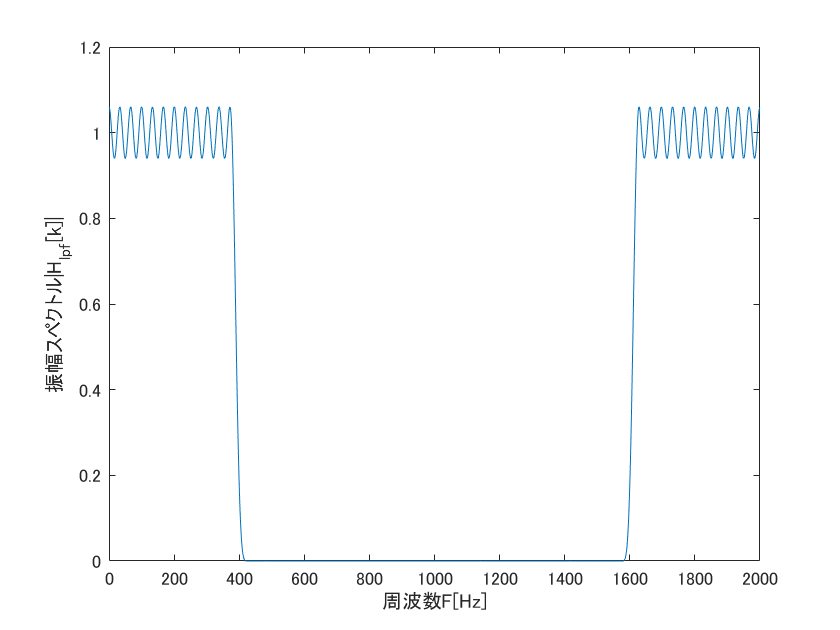
\includegraphics[width=\columnwidth]{figures/2-3lpf.png}
        \subcaption{ローパスフィルタ$h_{lpf}[n]$の振幅スペクトル$|H_{lpf}[k]|$}
        \label{fign:2-3lpf}
    \end{minipage}
    \begin{minipage}[t]{0.48\columnwidth}
        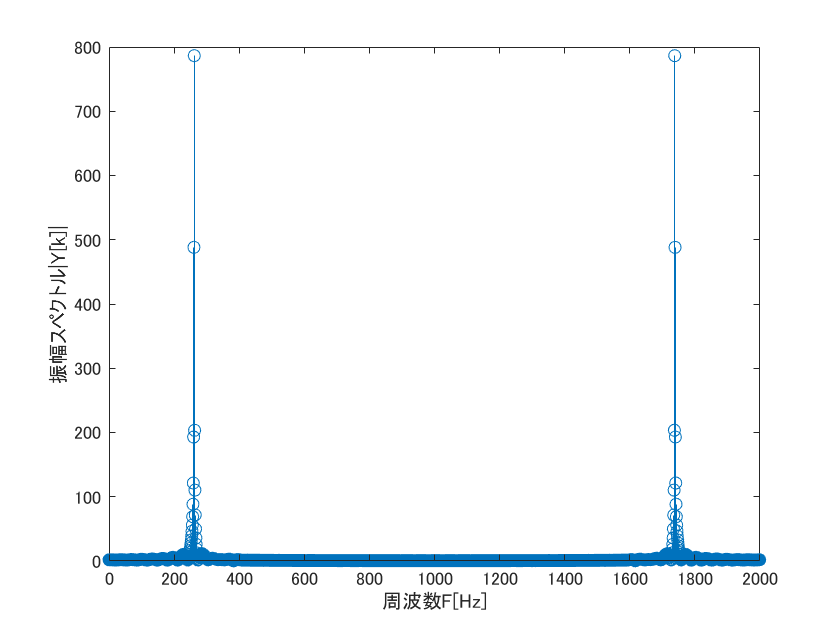
\includegraphics[width=\columnwidth]{figures/2-3y.png}
        \subcaption{畳み込み和$y[n]$の振幅スペクトル$|Y[k]|$}
        \label{fign:2-3y}
    \end{minipage}
    \end{center}
    \caption{\sout{課題2-3で得られたグラフ}
    遮断周波数400Hzのローパスフィルタを2000点FFTした振幅スペクトルと
    そのローパスフィルタを(ラ)の440Hzと(ド)の261.626Hzを合成した和音$x_{add}$に畳み込んで
    できたものをFFTした振幅スペクトル}
\end{figure}
\subsection*{考察}
図\ref*{fign:2-3lpf}より400Hzより低い周波数の振幅スペクトル
が大きくなっている.
図\ref*{fign:2-3y}と図\ref*{fign:2-2}より元の和信号$x_{add}[n]$
で見られた440Hzあたりのところにある振幅スペクトルが畳み込み和
$y[n]$では見られなくなっていて,$x_{2}[n]$の信号のように
なっている.
これは遮断周波数$F_{cut}=400$[Hz]のローパスフィルタの
畳み込みをしてローパスフィルタの振幅スペクトルが小さい周波数
だったのところが畳み込み和でも小さくなっている
からである.
したがって今回作成したローパスフィルタの働きは400Hz以下の周波数
だけを通して400Hzより大きい周波数を除くという働きであること
わかる.

\newpage
\section*{課題2-4}
\subsection*{実験結果(キャプションに追記あり)}
周波数仕様$Fs=2000$,遮断周波数$F_{cut}=400$[Hz]となるよう
通過域端周波数Fpassを399Hz,阻止域端周波数Fstopを401Hz
に設定してローパスフィルタ$h_{lpf2}[n]$ を設計した.
設計したローパスフィルタ$h_{lpf2}[n]$を$N=2000$点FFTし,
振幅スペクトル$|H_{lpf2}[k]|$を図\ref*{fign:2-3lpf2}
に示す.見やすさのために連続値として扱ってローパスフィルタを
プロットしている.
ローパスフィルタに合成和音$x_{add}[n]$を畳み込む.
そうして出来た畳み込み和$y[n]$を$N=2000$点FFTし,
振幅スペクトル$|Y[k]|$を図\ref*{fign:2-3y2}に示す.

周波数仕様$Fs=2000$,遮断周波数$F_{cut}=400$[Hz]となるよう
阻止域端周波数Fstopを390Hz,通過域端周波数Fpassを410Hz
に設定してハイパスフィルタ$h_{hpf}[n]$ を設計した.
設計したハイパスフィルタ$h_{hpf}[n]$を$N=2000$点FFTし,
振幅スペクトル$|H_{hpf}[k]|$を図\ref*{fign:2-4hpf}
に示す.見やすさのために連続値として扱ってハイパスフィルタを
プロットしている.
ハイパスフィルタに合成和音$x_{add}[n]$を畳み込む.
そうして出来た畳み込み和$y[n]$を$N=2000$点FFTし,
振幅スペクトル$|Y[k]|$を図\ref*{fign:2-4yh}に示す.

$x(t)=\sin(2\pi F_{a}t)$の$F_{a}$にドの261.626[Hz],
ファの349.228[Hz],ラの440.00[Hz]を入れた単音を合成した
合成和音$x_{add}$を生成しバンドパスフィルタをかける.
周波数仕様$Fs=2000$,
阻止域端周波数Fstop1を330Hz,通過域端周波数Fpass1を331Hz,
通過域端周波数Fpass2を360Hz,阻止域端周波数Fstop2を361Hz,
のバンドストップフィルタを設計した.
設計したバンドパスフィルタ$h_{bpf2}[n]$を$N=2000$点FFTし,
振幅スペクトル$|H_{bpf2}[k]|$を図\ref*{fign:2-4bpf}
に示す.見やすさのために連続値として扱ってバンドパスフィルタを
プロットしている.
バンドパスフィルタに合成和音$x_{add}[n]$を畳み込む.
そうして出来た畳み込み和$y[n]$を$N=2000$点FFTし,
振幅スペクトル$|Y[k]|$を図\ref*{fign:2-4yb}に示す.

\begin{figure}[h]
    \begin{center}
    \begin{minipage}[t]{0.48\columnwidth}
        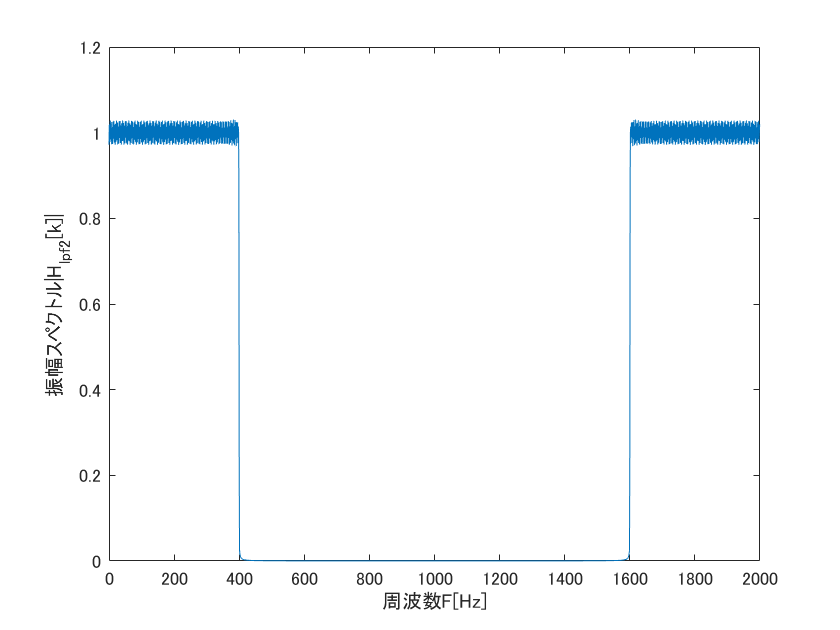
\includegraphics[width=\columnwidth]{figures/2-3lpf2.png}
        \subcaption{ローパスフィルタ$h_{lpf2}[n]$の振幅スペクトル$|H_{lpf2}[k]|$}
        \label{fign:2-3lpf2}
    \end{minipage}
    \begin{minipage}[t]{0.48\columnwidth}
        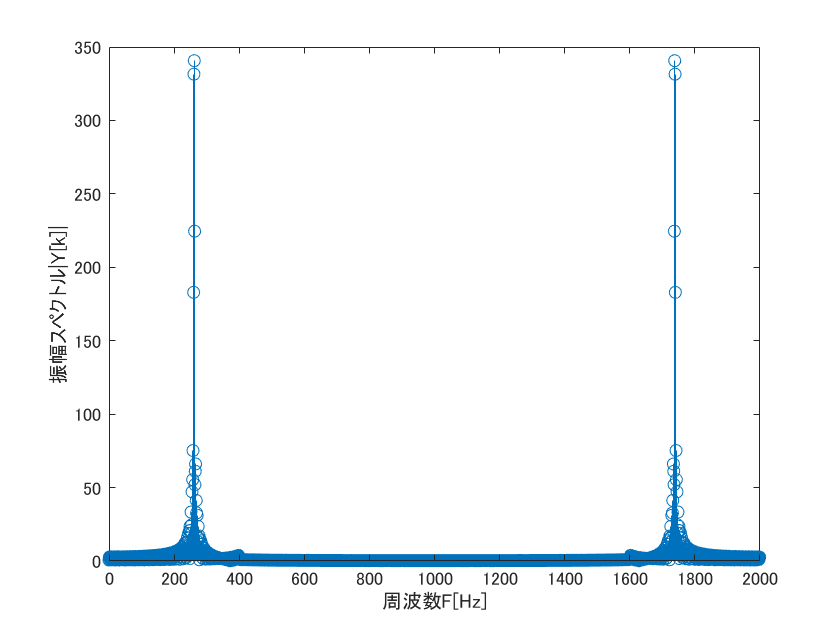
\includegraphics[width=\columnwidth]{figures/2-3y2.png}
        \subcaption{畳み込み和$y[n]$の振幅スペクトル$|Y[k]|$}
        \label{fign:2-3y2}
    \end{minipage}
    \end{center}
    \caption{(遮断周波数400Hzの理想に近い)ローパスフィルタ$h_{lpf2}$\sout{で得られたグラフ}
    をFFTした振幅スペクトルとそのローパスフィルタを(ラ)の440Hzと(ド)の261.626Hzを合成した和音$x_{add}$に畳み込んで
    できたものをFFTした振幅スペクトル}
\end{figure}
\begin{figure}[h]
    \begin{center}
    \begin{minipage}[t]{0.48\columnwidth}
        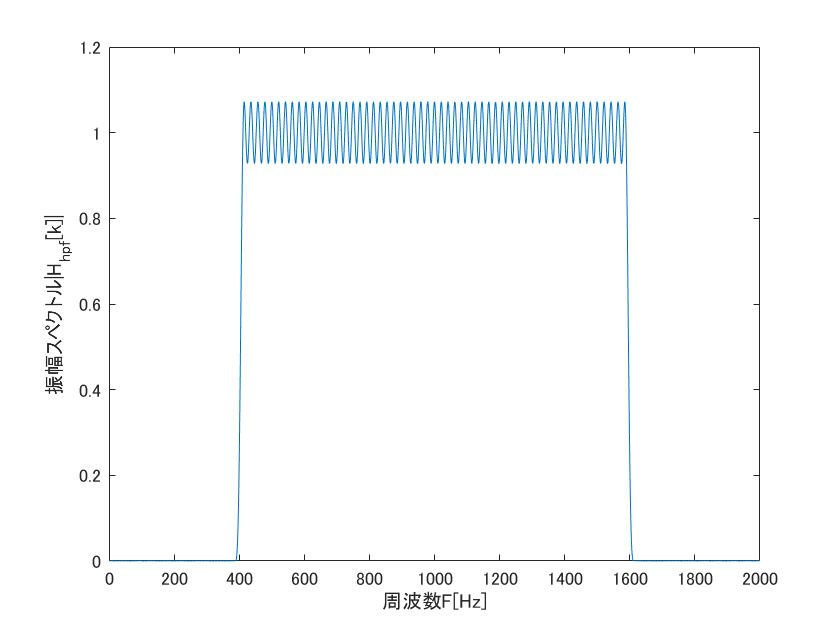
\includegraphics[width=\columnwidth]{figures/2-4hpf.png}
        \subcaption{ハイパスフィルタ$h_{hpf}[n]$の振幅スペクトル$|H_{hpf}[k]|$}
        \label{fign:2-4hpf}
    \end{minipage}
    \begin{minipage}[t]{0.48\columnwidth}
        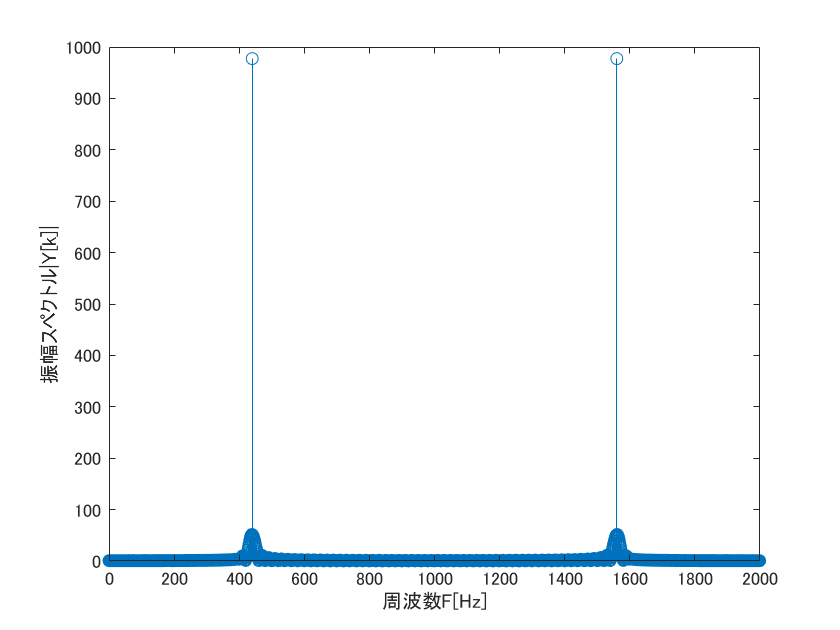
\includegraphics[width=\columnwidth]{figures/2-4yh.png}
        \subcaption{畳み込み和$y[n]$の振幅スペクトル$|Y[k]|$}
        \label{fign:2-4yh}
    \end{minipage}
    \end{center}
    \caption{(遮断周波数400Hzの)ハイパスフィルタ$h_{hpf}$\sout{で得られたグラフ}
    をFFTした振幅スペクトルとそのハイパスフィルタを(ラ)の440Hzと(ド)の261.626Hzを合成した和音$x_{add}$に畳み込んで
    できたものをFFTした振幅スペクトル}
\end{figure}
\begin{figure}[h]
    \begin{center}
    \begin{minipage}[t]{0.48\columnwidth}
        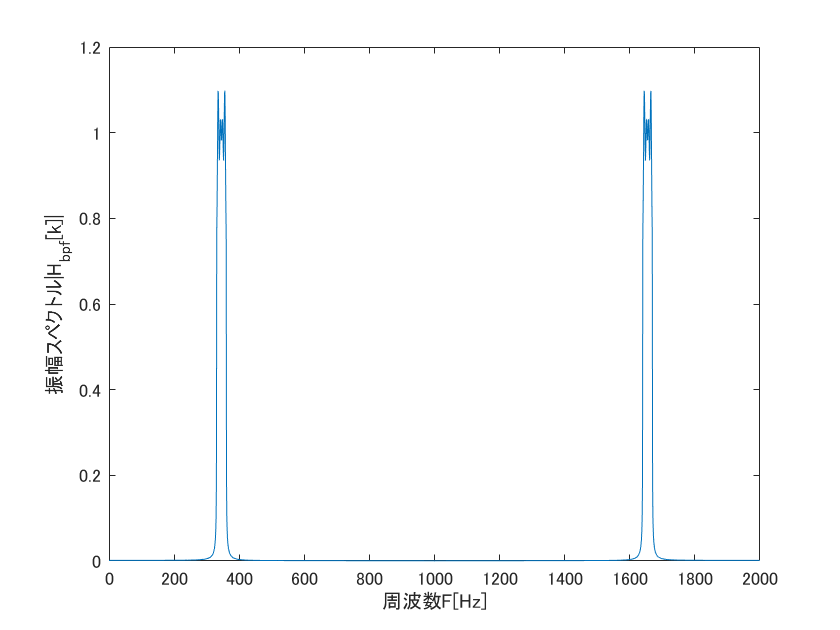
\includegraphics[width=\columnwidth]{figures/2-4bpf.png}
        \subcaption{バンドパスフィルタ$h_{bpf}[n]$の振幅スペクトル$|H_{bpf}[k]|$}
        \label{fign:2-4bpf}
    \end{minipage}
    \begin{minipage}[t]{0.48\columnwidth}
        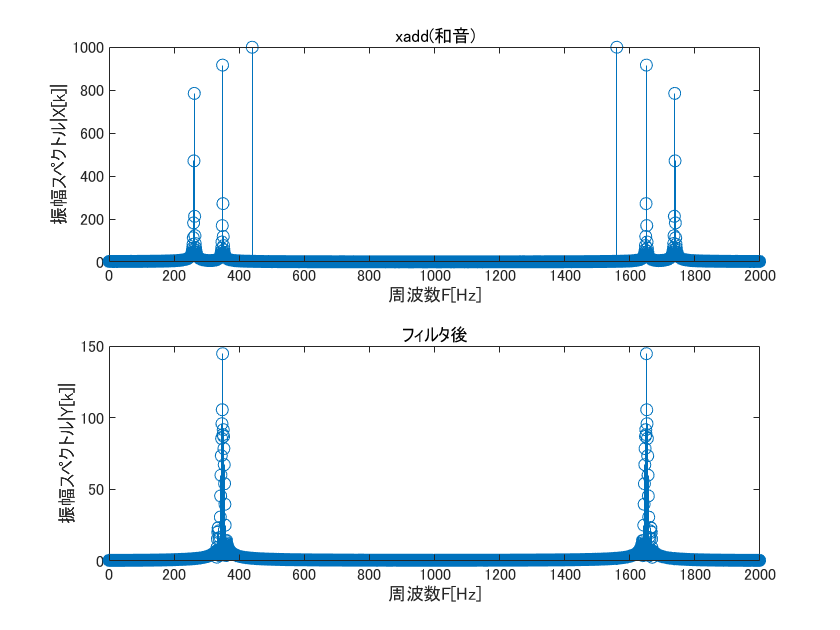
\includegraphics[width=\columnwidth]{figures/2-4yb.png}
        \subcaption{畳み込み和$y[n]$の振幅スペクトル$|Y[k]|$}
        \label{fign:2-4yb}
    \end{minipage}
    \end{center}
    \caption{330Hzから360Hzあたりを通すバンドパスフィルタ$h_{bpf}$\sout{で得られたグラフ}
    のFFTした振幅スペクトルとそのバンドパスフィルタを(ラ)の440Hzと(ド)の261.626Hzと
    (ファ)の349.228Hzを合成した和音$x_{add}$に畳み込んで
    できたものをFFTした振幅スペクトル}
\end{figure}
\newpage
 
\newpage
\subsection*{考察}
図\ref*{fign:2-3lpf2}と図\ref*{fign:2-3lpf}より遷移域が小さい
ローパスフィルタ$h_{lpf2}$のほうが400Hzより低い周波数のところで
は振幅スペクトルが1に近い値に固まっている.
これは$h_{lpf2}$のほうが遷移域が小さく複雑になっている
からである.
図\ref*{fign:2-3y2}と図\ref*{fign:2-3y}より
ローパスフィルタ$h_{lpf2}$のほうが261Hz辺りでの
振幅スペクトルがばらついている.
これは$h_{lpf2}$のほうが遷移域が小さく,フィルタが複雑になっているため
振幅スペクトルが存在しているところの付近の値も同じくらいの値が
畳み込みされているからである.
ドの音の周波数は小数のため,261Hzの値の隣の
周波数も振幅スペクトルが存在していてそれが遷移域が小さいと
畳み込み時に影響をあまり受けずに畳み込み和の
値が出てくるからである.
したがって遷移域を小さくすると理想のフィルタに近づき,通過する
周波数の振幅スペクトルへ与える影響が少なくすることができると
わかる.

図\ref*{fign:2-4hpf}より400Hzより高い周波数の振幅スペクトル
が大きくなっている.
図\ref*{fign:2-4yh}と図\ref*{fign:2-2}より元の和信号$x_{add}[n]$
で見られた261Hz付近にある振幅スペクトルが畳み込み和
$y[n]$では見られなくなっていて,$x_{1}[n]$の信号のように
なっている.
これは遮断周波数$F_{cut}=400$[Hz]のハイパスフィルタの
畳み込みをしてハイパフィルタの振幅スペクトルが小さい周波数
だったのところが畳み込み和でも小さくなっている
からである.
したがって今回作成したハイフィルタの働きは400Hz以上の周波数
だけを通して400Hzより小さい周波数を除くという働きであること
わかる.

図\ref*{fign:2-4bpf}より330Hzから360Hzのあたりの
周波数の振幅スペクトルが大きくなっている.
図\ref*{fign:2-4yb}より元の和信号$x_{add}[n]$
で見られた261Hz付近にある振幅スペクトル
や440Hz付近にある振幅スペクトルが畳み込み和
$y[n]$では見られなくなっている.
これはの330Hzから360Hzのバンドパスフィルタの
畳み込みをしてバンドパフィルタの振幅スペクトルが小さい周波数
だったのところが畳み込み和でも小さくなっている
からである.
したがって今回作成したバンドフィルタの働きは330Hzから360Hzの周波数
だけを通してそれ以外の周波数を除くという働きであること
わかる.

\newpage
\section*{課題2-A}
\subsection*{実験結果}
まず,原音声と原音声にノイズを付加したものを$N=2048$点FFTして
振幅スペクトルを確認する.二つの音声をFFTした振幅スペクトルの
結果を図\ref*{fign:2-Ao}に示す.図\ref*{fign:2-Ao}よりノイズ
は640Hzと768Hzの周波数で発生している.ノイズ除去のため
640Hzから768Hzまでの周波数を通さないバンドストップフィルタを
設計するという方針を立てて実行していく.周波数仕様$Fs=2048$,
通過域端周波数Fpass1を630Hz,阻止域端周波数Fstop1を632Hz,
阻止域端周波数Fstop2を770Hz,通過域端周波数Fpass2を772Hz,
のバンドストップフィルタを設計した.そしてノイズを除去した.
ノイズを除去した音声を$N=2048$点FFTしてできた振幅スペクトルは
図\ref*{fign:2-Az}に示す.
\begin{figure}[h]
    \begin{center}
    \begin{minipage}[t]{0.48\columnwidth}
        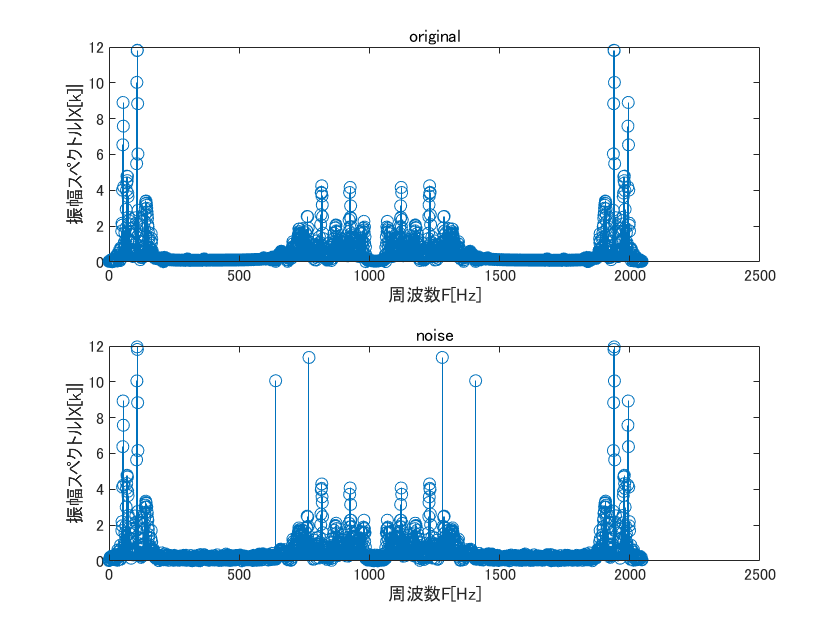
\includegraphics[width=\columnwidth]{figures/2-Ahikaku.png}
        \subcaption{原音声とノイズを付加した音声の比較}
        \label{fign:2-Ao}
    \end{minipage}
    \begin{minipage}[t]{0.48\columnwidth}
        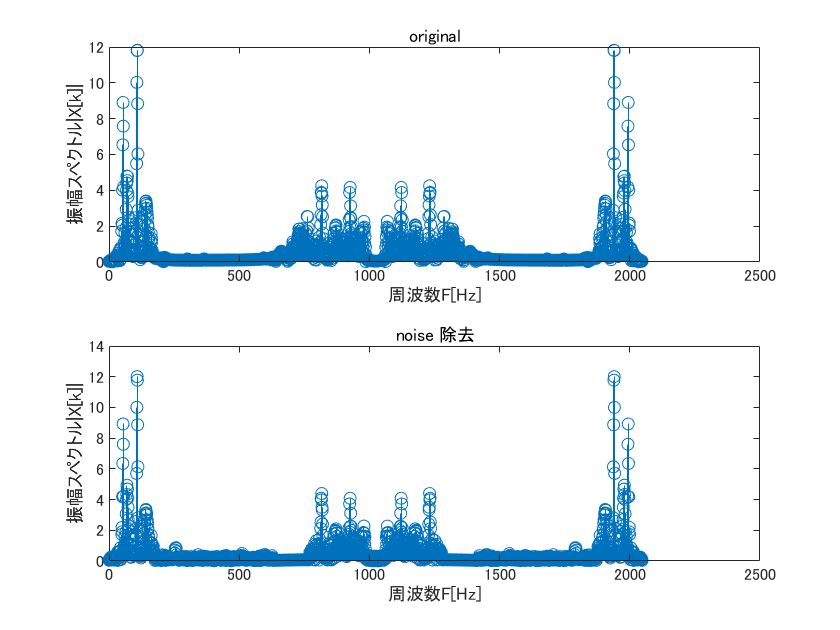
\includegraphics[width=\columnwidth]{figures/2-Azyokyo.png}
        \subcaption{原音声とノイズ除去後の音声の比較}
        \label{fign:2-Az}
    \end{minipage}
    \end{center}
    \caption{\sout{課題2-Aの実験結果}原音声とノイズとノイズを除去した音声の比較}
\end{figure}


\subsection*{考察}
図\ref*{fign:2-Az}より図\ref*{fign:2-Ao}のnoiseで見られるような
ノイズの振幅スペクトルが無くなり,原音声とあまり
変わらない振幅スペクトルを得られた.しかし,640Hzから768Hzまでの
間にあった小さな振幅スペクトルも無くなった.
音声を聞き比べると
dsp2\_noise.wavで聞こえたピーのような音が聞こえなくなった.
これはバンドストップフィルタがうまく働いたためである.
したがってノイズを付加された音声をFFTして振幅スペクトルを確認
して見つけた振幅スペクトルをなくすようにフィルタをかけると
ノイズ除去ができることがわかる.

\newpage
\section*{課題3-1}
\subsection*{実験結果}
図\ref*{fign:3-1-32}に4Hzを32点で標本化した離散時間信号$x_{32}[n]$
と$x_{32}[n]$を32点FFTした振幅スペクトル$|X_{32}[k]|$
の結果を示す.
図\ref*{fign:3-1-6}に4Hzを6点で標本化した離散時間信号$x_{6}[n]$
と$x_{6}[n]$を6点FFTした振幅スペクトル$|X_{6}[k]|$
の結果を示す.
\begin{figure}[h]
    \begin{center}
    \begin{minipage}[t]{0.48\columnwidth}
        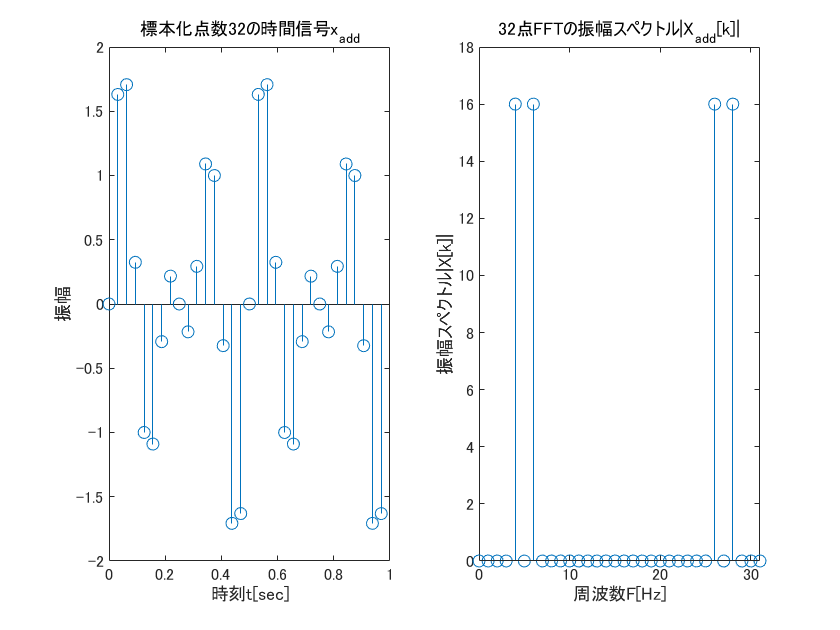
\includegraphics[width=\columnwidth]{figures/3-1-32.png}
        \subcaption{$x_{32}[n]$と
        その振幅スペクトル$|X_{32}[k]|$}
        \label{fign:3-1-32}
    \end{minipage}
    \begin{minipage}[t]{0.48\columnwidth}
        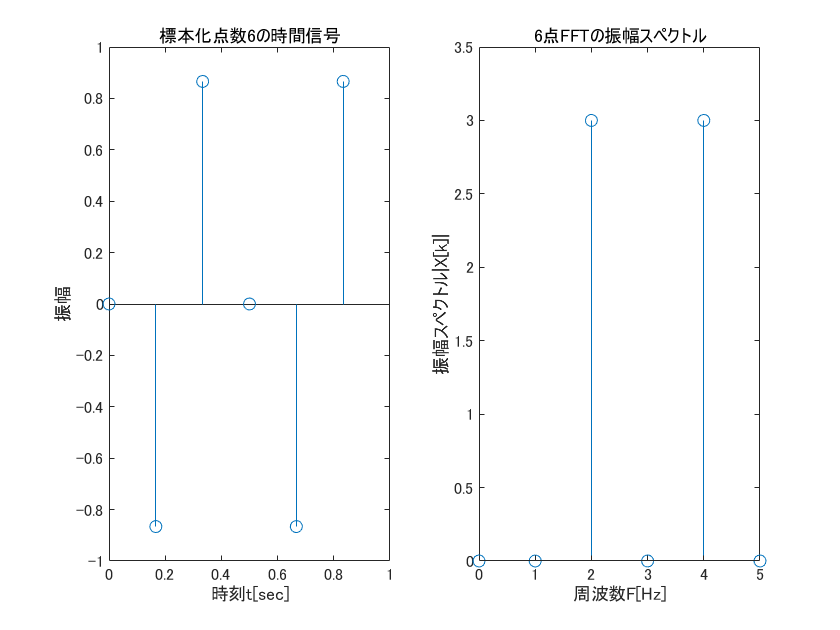
\includegraphics[width=\columnwidth]{figures/3-1-6.png}
        \subcaption{$x_{6}[n]$と
        その振幅スペクトル$|X_{6}[k]|$}
        \label{fign:3-1-6}
    \end{minipage}
    \end{center}
    \caption{4Hzの正弦波を32点で標本化した$x_{32}[n]$と6点で標本化した$x_{6}[n]$}
\end{figure}
\subsection*{考察}
図\ref*{fign:3-1-32}と図\ref*{fign:3-1-6}の時間信号を比較すると
32点で標本化した方は4Hzの正弦波に見えるが6点で標本化した
方は4Hzの正弦波に見えない.また,図\ref*{fign:3-1-6}の
振幅スペクトルより,今回の実験では4Hzの信号を使っているため
周波数$F=4$のところではじめて振幅スペクトルが立つはずだが,2のところに
立っている.これは今回の周波数は4Hzでナイキスト周波数
は$4\times 2 = 8$であったため
標本化周波数$F_{s}=6$では足りなかったためである.
したがって今回の周波数は4Hzでナイキスト周波数は$4\times 2 = 8$
より大きい周波数で標本化しなければ情報が消失してしまうこと
がわかる.



\newpage
\section*{課題3-2}
\subsection*{実験結果}
図\ref*{fign:3-2}に課題3-1で求めた離散時間フーリエスペクトル
$X_{32}[k],X_{6}[k]$を逆フーリエ変換して求めた時間信号
を示す.
\begin{figure}[h]
    \centering
    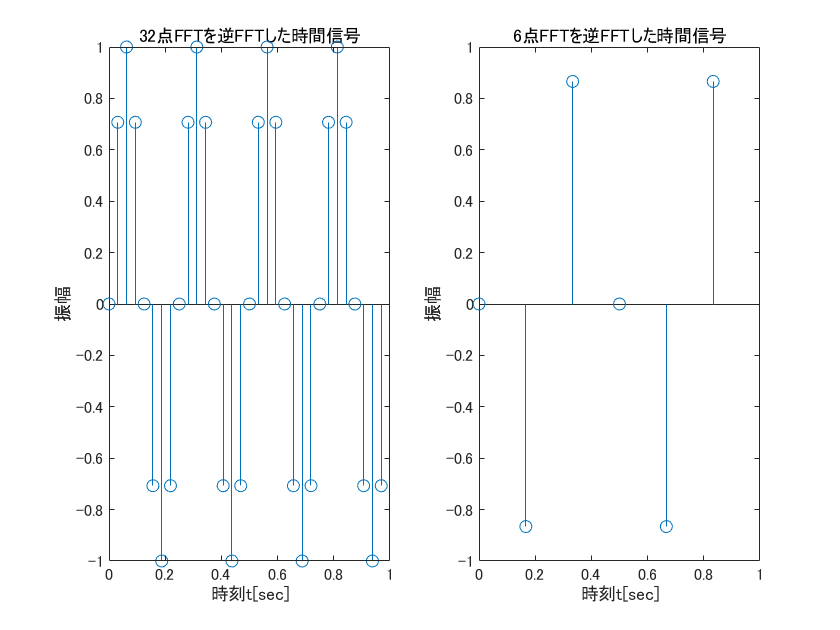
\includegraphics[width=0.9\linewidth]{figures/3-2.png}
    \caption{4Hzの正弦波を32点と6点で標本化した離散時間信号をフーリエ変換した
    離散時間フーリエスペクトル$X_{32}[k],X_{6}[k]$を
    逆フーリエ変換して求めた離散時間信号$x_{32}[n]$と$x_{6}[n]$}
    \label{fign:3-2}     
\end{figure}
\subsection*{考察}
図\ref*{fign:3-2}と図\ref*{fign:3-1-32}の時間信号を比較すると同じ
時間信号が得られている.また図\ref*{fign:3-2}と
図\ref*{fign:3-1-6}の時間信号を比較すると同じ
時間信号が得られている.これはフーリエ変換したものに逆フーリエ変換
を行ったためである.したがってフーリエ変換と逆フーリエ変換は
変換対であることがわかる.
図\ref*{fign:3-2}より標本化点数が6の方を逆フーリエ変換しても
得られた時間信号は4Hzの正弦波には見えない.これは標本化する
ときに情報が消失してしまっているためである.したがって
標本化定理を満たした条件で標本化する必要があることがわかる.

\newpage
\section*{課題3-3}
\subsection*{実験結果}
図\ref*{fign:3-3-org}に4Hzの正弦波と6Hzの正弦波を合成し,32点
で標本化した離散時間信号$x_{add}[n],(n=0,1,\dots,31)$と
$x_{add}[n]$を32点DFTした結果の振幅スペクトルを示す.
図\ref*{fign:3-3-cut}に合成した離散時間信号$x_{add}[n]$から
$n=7,\dots,29$までの23点を切り出した信号の離散時間信号
$x_{cut}[n]$と$x_{cut}[n]$を23点DFTした結果の振幅スペクトルを示す.
図\ref*{fign:3-3-mado}に切り出した離散時間信号$x_{cut}[n]$
に長さ23のハニング窓をかけた離散信号$x_{w}[n]$と
$x_{cut}[n]$を23点DFTした結果の振幅スペクトルを示す.


\begin{figure}[h]
    \begin{center}
    \begin{minipage}[t]{0.48\columnwidth}
        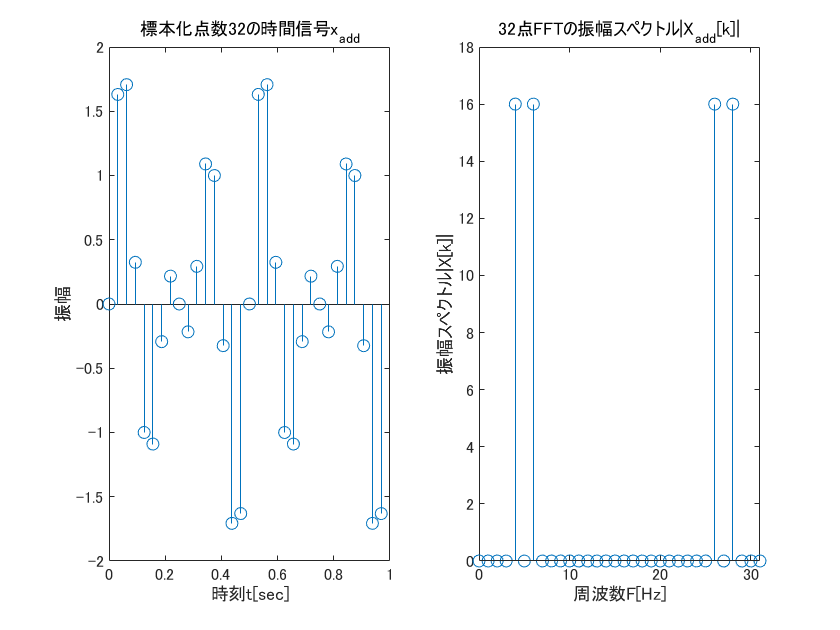
\includegraphics[width=\columnwidth]{figures/3-3-org.png}
        \subcaption{$x_{add}[n]$の離散時間信号と$x_{add}[n]$を32点DFTした振幅スペクトル}
        \label{fign:3-3-org}
    \end{minipage}
    \begin{minipage}[t]{0.48\columnwidth}
        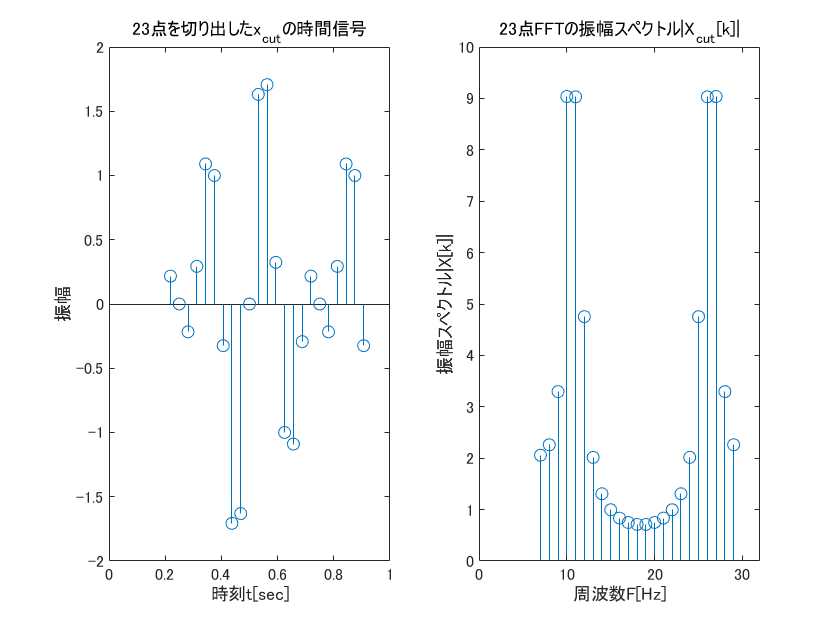
\includegraphics[width=\columnwidth]{figures/3-3-cut.png}
        \subcaption{$x_{add}[n]$の離散時間信号と$x_{add}[n]$を23点DFTした振幅スペクトル}
        \label{fign:3-3-cut}
    \end{minipage}
    \end{center}
    \caption{4Hzと6Hzの正弦波を合成した信号の32点で標本化した$x_{add}[n]$
    とその$n=7,\dots,29$を切り出した$x_{cut}[n]$}
\end{figure}
\begin{figure}[h]
    \centering
    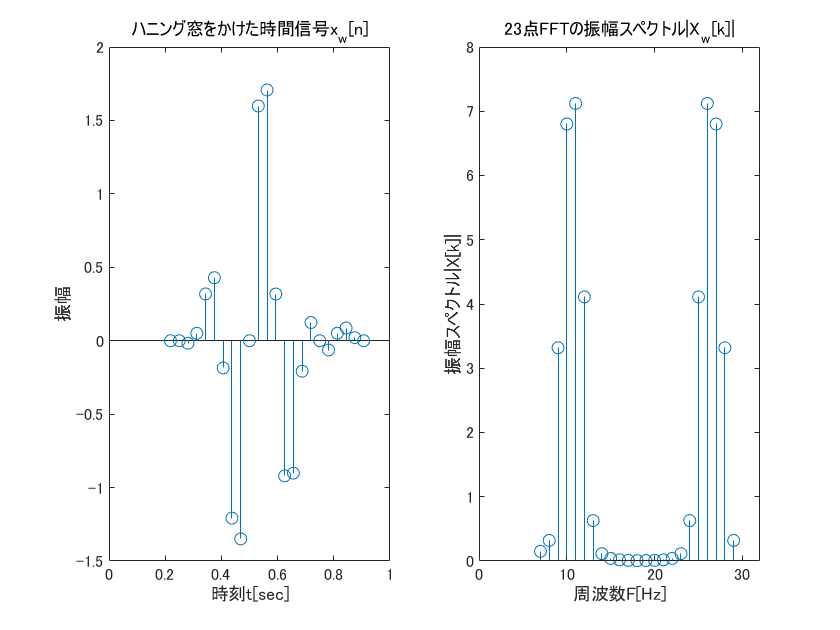
\includegraphics[width=0.9\linewidth]{figures/3-3-mado.png}
    \caption{切り出した離散時間信号$x_{cut}[n]$に長さ23のハニング窓をかけた
    離散信号$x_{w}[n]$と$x_{w}[n]$の23点DFTした振幅スペクトル}
    \label{fign:3-3-mado}
\end{figure}

\newpage
\subsection*{考察}
図\ref*{fign:3-3-org}と図\ref*{fign:3-3-cut}を比較すると
切り出す前は4Hzと6Hzのところに振幅スペクトルが立っているが
切り出した後は全てのところに振幅スペクトルが立っていて
複雑になっている.これはDFTというものは周期性を
仮定できることを前提としているため,中途半端に切り出すと
周期性が崩れてしまったためである.したがってDFT
は非周期信号に使うことはできないという問題があることがわかる.
図\ref*{fign:3-3-cut}と図\ref*{fign:3-3-mado}を比較すると
時間領域ではハニング窓をかけると信号の端が0になっている.
また周波数領域ではハニング窓をかけると高周波数成分がなくなって
いる.これはハニング窓をかけて無理やり端を0にして周期性を
持たせたためである.したがって窓関数は非周期信号に信号を
持たせて,いびつな形を表現するための高周波数成分を不要に
させるという影響を与えているということがわかる.


\newpage
\section*{課題3-A}
\subsection*{実験結果}
追加課題1-Aで作成した短形波を$N=200$にして作成した短形波
を$N=200$にしてFFTし,そのまま逆フーリエ変換で戻した結果と
第2回の実験でしたように
遮断周波数50Hzのローパスフィルタを作成し,それを作成した短形波に
かけてから逆フーリエ変換して戻した結果を図\ref*{fign:3-A}に示す.

\begin{figure}[h]
    \centering
    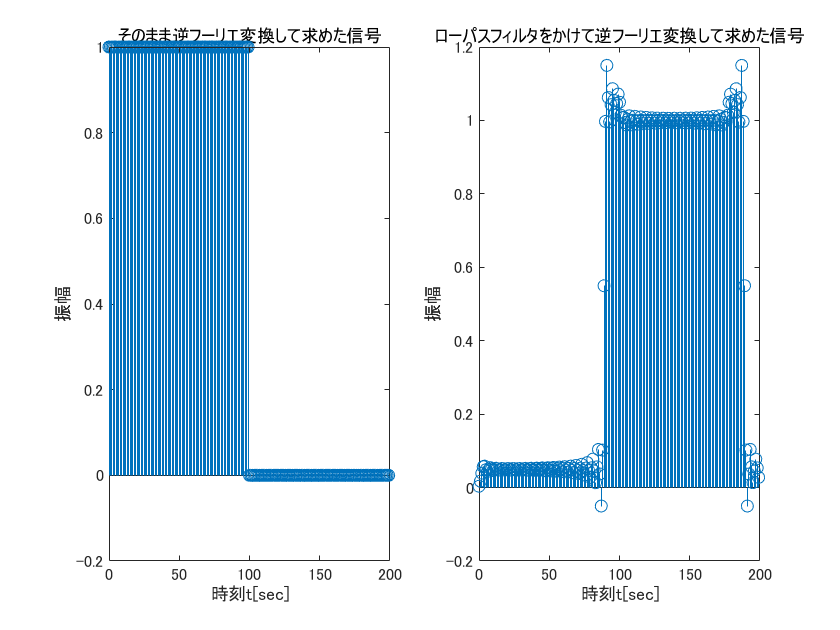
\includegraphics[width=0.9\linewidth]{figures/3-A.png}
    \caption{$N=200$とし,
$0\leq t \leq N/2$の時$y(t)=1$,$t>N/2$の時
$y(t)=0$の短形波$y(t)$
        をFFTして逆FFTした時間信号と遮断周波数50Hzのローパスフィルタをかけて
    FFTして逆FFTした時間信号}
    \label{fign:3-A}
\end{figure}

\subsection*{考察}
図\ref*{fign:3-A}よりそのまま逆フーリエ変換した方は
もとの短形波が出てくるのに対してローパスフィルタをかけた方
は0と1が逆になっている.また周期が少し短くなっている.
これはローパスフィルタをかけたためである.したがって
ローパスフィルタは高周波数成分を除くので短形波にある高周波数成分
がいつ0になるのか1になるのかに影響を与えていて高周波数成分を
なくすとこのような違いになると考えられる.

\newpage
\section*{おわりに}

信号処理の部分を深く理解していないため何をやっているか全く
分からないままやっていて大変だった.

第1回の時よりは理解が深まって何しているか部分的には分かっている
つもりになっているが,難しかった.今回気づいたがレポートの名前を
APL\_DSP\_学修番号\_名前にしなければならないのにLaTeXのテンプレート
がapl\_dsp\_xxxxxxxx\_name.texになっているのは許せない.

離散時間信号と離散信号の文字がたくさんあってなにがなんだか分からなく
なってしまった.レポートの書き方をたくさん学べて良かった.
最後の追加課題でもっと意味が分からなくなってしまった.
特に追加課題とかもう少し詳しく書いてほしいとおもった.
第2回の実験ではもとの信号にローパスフィルタをかけているが
第3回ではFFTしたあとにかけているふうにも取れる気がします.
\begin{thebibliography}{99}
    \bibitem{shiraki2024}
    参考にした書籍,サイト,文献を記載せよ
    
\end{thebibliography}

\end{document}